\chapter{Estudio previo}\label{chapter:estudio_previo}

Este capítulo se divide en dos partes. En la primera parte se estudian los fundamentos del aprendizaje por refuerzo, donde se definen conceptos clave y se analiza cómo se aplican en la práctica estudiando los métodos pertinentes, con el objetivo de entender cómo funcionan los algoritmos que se utilizarán finalmente en el desarrollo del proyecto.

Es posible que para entender algunos de estos conceptos en su totalidad sea necesario tener un conocimiento previo sobre el aprendizaje profundo, por lo que se recomienda el libro \emph{Deep Learning} \cite{Goodfellow-et-al-2016} como recurso adicional.

En la segunda parte se exploran las características de \emph{Unity ML-Agents Toolkit}, dando énfasis a aquellas herramientas y funcionalidades que son relevantes para la fase de desarrollo. En particular, se comentan los componentes clave de ML-Agents y los métodos de entrenamiento que se ponen en práctica en este proyecto.

\section{Estructura de un problema de RL}

\subsection{Proceso de decisión de Márkov}

En la Sección \ref{section:conceptos} se propuso una definición tanto formal como informal del proceso por el que pasa un agente de RL. En matemáticas, este proceso se conoce como el proceso de decisión de Márkov (MDP). De hecho, cuando un problema puede ser descrito como un MDP, un algoritmo de RL puede ser una buena elección para resolverlo. Normalmente, un MDP se define como una 5-tupla $(S, A, R, P, \gamma)$ donde:

\begin{enumerate}
    \item[\textbullet] $S$ es el conjunto de todos los estados del entorno.
    \item[\textbullet] $A$ es el conjunto de todas las acciones que puede realizar un agente.
    \item[\textbullet] $R : S \times A \times S \rightarrow \mathbb{R}$ es la función de recompensa $r_t = R(s_t, a_t, s_{t+1})$ donde $r_t$ es la recompensa recibida tras pasar del estado $s_t$ al estado $s_{t+1}$ debido a la acción $a_t$.
    \item[\textbullet] $P : S \times A \rightarrow P(S)$ es la función de probabilidad de transición, siendo $P(s'|s, a)$ la probabilidad de llegar al estado $s'$ si se empieza en el estado $s$ y se toma la acción $a$.
    \item[\textbullet] $\gamma$ es el factor de descuento que determina la importancia de las recompensas futuras en relación con las más cercanas.
\end{enumerate}

Dependiendo del contexto de un problema, en ocasiones se utilizan variaciones de esta tupla en las que se sustituye el factor de descuento $\gamma$ con una distribución del estado inicial $p_0$, o bien se define únicamente con las variables $S, A, R$ y  $P$. Por ejemplo, en entornos en los que, dependiendo del estado inicial, la secuencia de acciones óptima puede variar notablemente, sería relevante definir la distribución del estado inicial.

El nombre de este proceso hace referencia a la propiedad de Márkov: las transiciones dependen únicamente del estado y la acción más reciente, y no del historial de estados y acciones pasadas. Esta propiedad es fundamental para los problemas de RL, ya que permite simplificar la representación de estados y, de esta manera, reducir la complejidad computacional.

\subsection{Espacio de observaciones y estados}

El espacio de observaciones y estados es la información que recibe un agente del entorno. Un estado $s$ es una descripción completa del estado del mundo, sin información oculta. Una observación $o$, en cambio, es una descripción parcial del mundo la cual puede omitir alguna información, dependiendo de cómo se haya modelado el problema.

Los estados y las observaciones se suelen representar con vectores, matrices o tensores. Por ejemplo, el estado de un juego de Atari se puede representar como una matriz RGB con el valor de cada píxel; el estado de un brazo robot se puede representar como un vector con las posiciones y velocidades angulares de sus ejes.
En la práctica, la notación estándar $s$ hace referencia a observaciones y estados indistintamente, ya que se sobrentiende de qué se trata realmente a partir del contexto del problema.

\subsection{Espacio de acciones}

El espacio de acciones es el conjunto de acciones válidas que se pueden realizar en un entorno determinado. En algunos entornos, como Atari o el ajedrez, el espacio de acciones es discreto, ya que el número de movimientos que puede realizar un agente es limitado. En otros, como por ejemplo el de un agente que controla un robot que se mueve en un mundo físico, el espacio de acciones es continuo, ya que acciones como por ejemplo el ángulo de giro se expresan mediante valores reales y por lo tanto es infinito.

\subsection{Retorno, episodios y el factor de descuento}

El objetivo de un agente es maximizar la recompensa acumulada que recibe a largo plazo. Dada una secuencia de recompensas recibidas a partir de un instante $t$, denotada $R_{t+1}$, $R_{t+2}$, $R_{t+3}$, ..., en general, el aspecto que se busca maximizar es el retorno esperado (o recompensa acumulada esperada), donde el retorno $G_t$ se define como:
\begin{equation}
\label{retorno_finito}
    G_t = R_{t+1} + R_{t+2} + R_{t+3} + ... + R_{T} = \sum_{k=t+1}^{T} R_{k}
\end{equation}
donde $T$ es el último instante de la secuencia.

Este planteamiento tiene sentido cuando existe una noción temporal de inicio y fin en el entorno, es decir, cuando la interacción entre el agente y el entorno puede dividirse en subsecuencias, conocidas como episodios. Cada episodio termina en un estado final, seguido de un reinicio hacia un estado inicial estándar o una instancia de una distribución de estados iniciales.

Por otra parte, hay entornos en los que la interacción entre el agente y el entorno no se puede dividir en episodios, sino que continúa infinitamente, conocidos como entornos continuos.

En los entornos continuos, el planteamiento de la Ecuación \ref{retorno_finito} resulta ser un problema ya que $T = \infty$, por lo que el objetivo a maximizar podría ser infinito. El concepto que se introduce para solucionar este problema es el factor de descuento $\gamma \in [0, 1]$, dando lugar al retorno con descuento con horizonte infinito.

\newpage

El retorno con descuento con horizonte infinito consiste en la suma de todas las recompensas obtenidas por el agente, pero descontadas según cómo de lejos en el futuro se hayan obtenido:
\begin{equation}
    G_t = R_{t+1} + \gamma R_{t+2} + \gamma^2 R_{t+3} + ... = \sum_{k=0}^{\infty} \gamma^k R_{t+k+1}
    \label{retorno_infinito}
\end{equation}

La intuición detrás del uso del factor de descuento consiste en que es más probable obtener aquellas recompensas más cercanas que no las más lejanas, debido a la incertidumbre acerca del futuro en un sistema dinámico, por lo que se le atribuye más valor a estas primeras. Cuando $\gamma = 0$, el agente solo tiene en cuenta las recompensas inmediatas. En cambio, cuando $\gamma$ se aproxima a 1, también da relevancia a las recompensas futuras, pero no tanta como a las inmediatas.

Matemáticamente, cuando $\gamma < 1$, la suma infinita de la Ecuación \ref{retorno_infinito} puede converger hacia un número finito, lo cual simplifica su uso.

\section{RL basado en modelos y sin modelos}

Una vez entendido cómo se estructura un problema de RL, lo siguiente es estudiar cómo se utilizan estos conceptos en el entrenamiento de agentes, y saber qué clase de algoritmos se utilizan para este fin.

En la clasificación de algoritmos de RL, la principal distinción parte de preguntarse si el agente tiene acceso a un \emph{modelo del entorno}. Un modelo del entorno consiste en la representación de la dinámica de un entorno, es decir, una función capaz de predecir la transición de estados y la recompensa que conlleva llegar a ciertos estados. Aunque este TFG se centra exclusivamente en el RL sin modelos, por completitud, conviene tener también una idea general sobre el RL basado en modelos.

En el RL basado en modelos, un agente planifica por adelantado su trayectoria, explorando todo un espacio de posibles estados y acciones, es decir, el modelo, para elegir de manera explícita qué opciones generan una recompensa acumulada óptima. El modelo puede ser dado o aprendido, pero debido a que usualmente es complicado construir un modelo exacto del entorno, suele ser el agente quien aprende una aproximación del modelo durante el entrenamiento.

Aunque los métodos basados en modelos necesitan pocas muestras, aprender un modelo no es sencillo y es intensivo desde un punto de vista computacional, ya que requieren más capacidad de procesamiento y memoria. Estos métodos suelen utilizarse en entornos bien definidos y no cambiantes. Un ejemplo de métodos basados en modelos es AlphaZero, un algoritmo capaz de jugar a ajedrez, shogi y go, desarrollado por DeepMind.

La contraparte de los métodos basados en modelos son los métodos sin modelos, los cuales no requieren un modelo del entorno para funcionar. En su lugar, utilizan un enfoque de prueba y error para tratar de lograr una estrategia óptima. Durante el proceso de aprendizaje, mediante la experiencia (es decir, la interacción del agente con el entorno), el agente estima una ``función de valor'' o una ``política'' (conceptos que se explican más adelante) que una vez entrenadas las utiliza para determinar qué acciones realizar.

Los métodos sin modelos, a pesar de requerir una gran cantidad de muestras, tienden a ser más fáciles de implementar y entrenar. Suelen utilizarse en entornos grandes, cambiantes y que no se pueden describir fácilmente.

\begin{figure}[H]
    \centering
    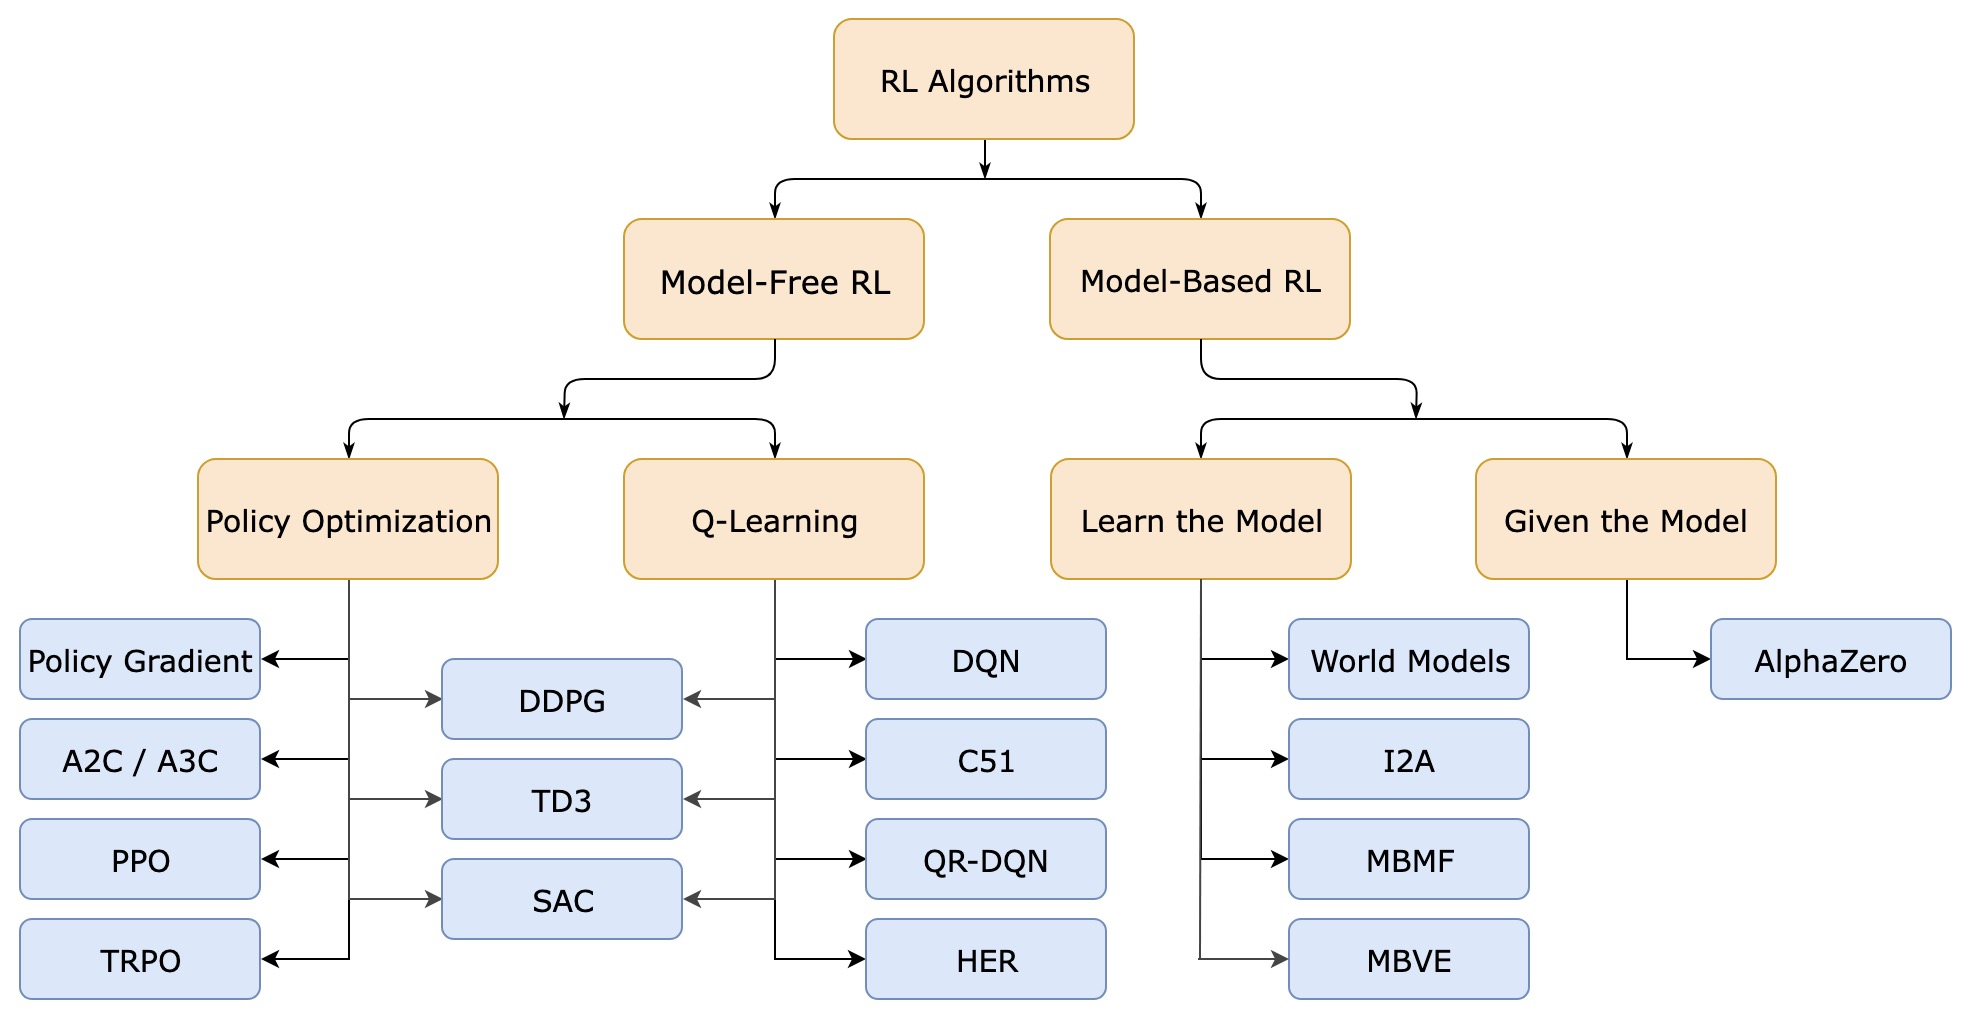
\includegraphics[width=15cm]{figures/taxonomia-rl.jpg}
    \caption[Taxonomía de algoritmos de RL]{Taxonomía de algoritmos de RL. (Fuente: \parencite{openai-rl})}
    \label{taxonomia-rl}
\end{figure}

\section{Métodos sin modelos}

Recordando la definición formal de RL de la Sección \ref{section:conceptos}, cuando un agente percibe un estado $s_t \in S$, selecciona una acción $a \in A(s_t)$  y pasa al estado $s_{t+1}$. Esta selección se realiza de acuerdo a la política del agente $\pi$, una funcion que indica qué acción realizar cuando el agente se encuentra en un determinado estado. El objetivo final en RL es, por lo tanto, encontrar una política óptima $\pi^{*}$, es decir, la política que maximiza el retorno esperado cuando el agente actúa de acuerdo a esta.

La política óptima se puede obtener de dos maneras:
\begin{enumerate}
    \item[-] Directamente, cuando el agente aprende una política, es decir, qué acción realizar dado el estado actual: métodos basados en la política.
    \item[-] Indirectamente, cuando el agente aprende una función de valor, es decir, cuán valioso es un estado, y elige las acciones que le lleven al mayor número de estados valiosos: métodos basados en el valor. 
\end{enumerate}

Por lo tanto, dentro de los métodos sin modelos, es posible hacer otra distinción según si se basan en el valor o en la política.

\subsection{Métodos basados en el valor}

En los métodos basados en el valor, el agente aprende una función de valor que devuelve el retorno esperado que puede obtener cuando empieza en cierto estado y actúa de acuerdo a una política hasta el final.

\newpage

La política en los métodos basados en el valor no es algo que se pueda aprender, a diferencia de la política en los métodos basados en la política, como se verá más adelante. En los métodos basados en el valor, la política se trata de una función predefinida a mano y suele consistir en una estrategia sencilla. Por ejemplo, una vez aprendida la función de valor, una política que podría adoptar el agente sería el de elegir siempre la acción que más valor le genere. A esta política se le llama política \emph{greedy}.

La idea de los métodos basados en el valor es que el agente, a medida que interactúa con el entorno, vaya afinando esta función de valor para que, una vez termine el entrenamiento, pueda utilizarla como guía para determinar la trayectoria a seguir.

Hay dos tipos de funciones de valor:
\begin{enumerate}
    \item[-] La función de valor del estado $v_{\pi}(s)$, la cual devuelve el retorno esperado cuando el agente empieza en el estado $s$ y actúa siguiendo una política $\pi$ hasta el final.
        \begin{equation}
            v_{\pi}(s) = \mathbb{E}_{\pi} \left[ G_t \, \middle| \, S_t = s \right] = \mathbb{E}_{\pi} \left[ \sum_{k=0}^{\infty} \gamma^k R_{t+k+1} \, \middle| \, S_t = s \right]
            \label{state-value}
        \end{equation}
    \item[-] La función de valor de la acción $q_{\pi}(s, a)$, la cual devuelve el retorno esperado cuando el agente empieza en el estado $s$, realiza una acción $a$, y sigue una política $\pi$ hasta el final.
        \begin{equation}
            q_{\pi}(s, a) = \mathbb{E}_\pi \left[ G_t \, \middle| \, S_t = s, A_t = a \right] = \mathbb{E}_\pi \left[ \sum_{k=0}^{\infty} \gamma^k R_{t+k+1}  \, \middle| \, S_t = s, A_t = a \right] 
            \label{action-value}
        \end{equation}
\end{enumerate}

Las funciones de valor introducen un orden parcial sobre las distintas políticas: una política $\pi$ es mejor o igual que otra política $\pi'$ cuando su retorno esperado es mayor o igual que el de la política $\pi'$ para todos los estados. Formalmente, para una función de valor del estado $v_\pi(s)$, y de manera similar para una función de valor de la acción $q_\pi(s,a)$, $\pi \geq \pi'$ si y solo si $v_\pi(s) \geq v_{\pi'}(s)$ para todos los estados $s \in S$. Por lo tanto, siempre habrá al menos una política que es mejor o igual que el resto de políticas, es decir, una política óptima $\pi^{*}$.

Encontrar la función de valor óptima, es decir, la función que maximiza el retorno esperado, daría lugar a obtener una política óptima:
\begin{equation}
    v^{*}(s) = \max_{\pi} v_{\pi}(s)
\end{equation}
\begin{equation}
    q^{*}(s,a) = \max_{\pi} q_{\pi}(s, a)
\end{equation}

\subsubsection{Ecuación de Bellman}

En la práctica, estimar las funciones de valor con las Ecuaciones \ref{state-value} y \ref{action-value} tal y como estan definidas puede llegar a ser algo tedioso: primero porque para el cálculo del valor de un solo estado es necesario hacer un recorrido de toda una secuencia de recompensas y estados; y segundo porque son funciones que deben estar definidas para todos los estados posibles, por lo que muchos de estos cálculos se acaban repitiendo, ya que algunos recorridos son subconjuntos de otros.

Para tratar de simplificar las funciones de valor, se siguen los principios de la programación dinámica para dividir el problema de calcular el retorno $G_t$, el cual es bastante complejo, en subproblemas más pequeños y manejables.

A partir de la función de retorno $G_t$ (Ecuación \ref{retorno_infinito}), se puede definir una relación recursiva entre la recompensa inmediata y las recompensas futuras:
\begin{equation}
\begin{split}
    G_t &= R_{t+1} + \gamma R_{t+2} + \gamma^2R_{t+3} + \gamma^3R_{t+4} + ... \\
    &= R_{t+1} + \gamma (R_{t+2} + \gamma R_{t+3} + \gamma^2R_{t+4} + ...) \\
    &= R_{t+1} + \gamma G_{t+1} \\
\end{split}
\end{equation}

Sustituyendo esta relación en la función de valor del estado $v_{\pi}(s)$:
\begin{equation}
\begin{split}
    v_{\pi}(s) &= \mathbb{E}_{\pi} \left[ G_t \, \middle| \, S_t = s \right] \\
    &= \mathbb{E}_{\pi} \left[ R_{t+1} + \gamma G_{t+1} \, \middle| \, S_t = s \right] \\
    &= \sum_{a} \pi \left( a \, \middle| \, s \right) \sum_{s'} \sum_{r} p \left( s', r \, \middle| s, a\, \right) \bigg[r + \gamma \mathbb{E}_{\pi} \left[ G_{t+1} \, \middle| \, S_{t+1}=s' \right] \bigg] \\
    &= \sum_{a} \pi \left( a \, \middle| \, s \right) \sum_{s', r} p \left( s', r \, \middle| s, a\, \right) \bigg[r + \gamma v_{\pi}(s') \bigg] \\
\end{split}
\label{eq:bellman-state}
\end{equation}

Similarmente, para la función de valor de la acción $q_\pi(s, a)$:
\begin{equation}
    q_{\pi}(s, a) = \sum_{s', r} p(s', r \,|\, s, a) \left[r + \gamma \sum_{a'} \pi(a' \,|\, s') q_{\pi}(s', a')\right]
\end{equation}

Estas son las ecuaciones de Bellman para las funciones de valor del estado y de la acción. Siguiendo una estructura recursiva, se descompone el valor de un estado o un par estado-acción en la suma de una recompensa inmediata más el valor descontado del siguiente estado. De esta manera, para calcular el retorno esperado de un estado o un par estado-acción basta con tener información del estado actual y del estado siguiente, en lugar de toda una secuencia de estados, resultando en un proceso mucho más eficiente.

\subsubsection{Estrategias de aprendizaje: Monte Carlo y Diferencia Temporal}

Hasta ahora se ha hablado de qué son las funciones de valor, para qué se utilizan y cómo se calculan. El cálculo, sin embargo, no es un proceso que se pueda ejecutar directamente haciendo un recorrido exhaustivo sobre todas las posibles secuencias de estados, hasta hallar la función de valor que mejor describa la bondad de cada estado o par estado-acción. Más bien, se trata un proceso iterativo en el que el agente, a medida que interactúa con el entorno, actualiza el valor de cada estado según la cantidad de recompensas que haya obtenido. A este proceso se le llama entrenamiento.

Durante el entrenamiento, se utilizan distintas estrategias de aprendizaje que, en esencia, determinan la frecuencia con la que se actualizan los valores de cada estado. En esta sección se estudian las estrategias de aprendizaje de Monte Carlo y Diferencia Temporal.
\newpage
En la estrategia de Monte Carlo, el agente actualiza la función de valor al final de un episodio, utilizando el retorno del episodio $G_t$ como objetivo:
\begin{equation}
    v(s_t) \leftarrow v(s_t) + \alpha [G_t - v(s_t)]
    \label{mc-state}
\end{equation}
\begin{equation}
    q(s_t, a_t) \leftarrow q(s_t, a_t) + \alpha [G_t - q(s_t, a_t)]
    \label{mc-action}
\end{equation}
donde $\alpha$ es la tasa de aprendizaje (\emph{learning rate}). De esta manera, tras cada episodio, el valor de los estados recorridos se van actualizando dependiendo de cuán mejor o peor haya sido el retorno obtenido a partir del estado correspondiente, incrementándose o decrementándose dependiendo de la tasa de aprendizaje $\alpha$, hasta converger a una función de valor óptima.

%\begin{figure}[H]
%    \centering
%    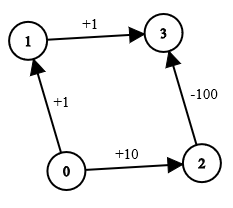
\includegraphics[width=5cm]{figures/graph.png}
%    \caption[Ejemplo simple de un entorno de RL]{Ejemplo simple de un entorno de RL (Fuente: elaboración propia)}
%    \label{simple-graph}
%\end{figure}

%Por ejemplo, dado un entorno simple definido por el grafo direccional que se muestra en la Figura \ref{simple-graph}, en el que el agente siempre empieza en el vértice 0 como estado inicial, y cuyo objetivo es llegar hasta el vértice 3, maximizando la recompensa obtenida por moverse de un vértice a otro, definido por el peso de cada arista, la idea sería que tras el entrenamiento, el valor de estar en el vértice 1 sea mayor que estar en el vértice 2, es decir, $v(s_1) > v(s_2)$. El agente, a priori, solo puede observar la recompensa que puede obtener desde el vértice en el que se encuentra, por lo que inicialmente se decantaría más por ir hacia el vértice 2, ya que la recompensa inmediata que recibe es mayor que la que recibe cuando se desplaza hacia el vértice 1. Sin embargo, desde el vértice 2, el agente descubre que para llegar hasta el objetivo debe recibir una penalización enorme. Tras llegar al vértice final, termina el episodio y actualiza la función de valor acorde al retorno obtenido: como que la recompensa acumulada de la secuencia $0 \rightarrow 2 \rightarrow 3$ ha sido negativa, el valor de estar en el vértice 2 decrementaría según la tasa de aprendizaje. De este modo, tras una serie de episodios, el agente acabará aprendiendo una función de valor que le indicará que el camino óptimo pasa por el vértice 1, por mucho que la recompensa inmediata por ir al vértice 2 sea mayor.

En la estrategia de Diferencia Temporal, a diferencia de la estrategia de Monte Carlo, el agente actualiza la función de valor en cada paso (o iteración). Esta vez, el agente no dispone de ningún retorno $G_t$, ya que no experimenta un episodio entero. En su lugar, estima el retorno $G_t$ con la suma de la recompensa inmediata $R_{t+1}$ más el valor descontado del siguiente estado: 
\begin{equation}
    v(s_t) \leftarrow v(s_t) + \alpha [R_{t+1} + \gamma v(s_{t+1}) - v(s_t)]
    \label{eq:mc-state}
\end{equation}
\begin{equation}
    q(s_t, a_t) \leftarrow q(s_t, a_t) + \alpha [R_{t+1} + \max_{a} q(s_{t+1}, a) - q(s_t, a_t)]
    \label{eq:mc-action}
\end{equation}
Utilizar la estimación del retorno se conoce como \emph{bootstrapping}, ya que se aproxima la función de valor utilizando estimaciones de valores ya existentes, $v(s_{t+1})$ o $q(s_{t+1}, a_{t+1})$, en lugar de una muestra completa $G_t$. La diferencia entre la aproximación del retorno y el valor del estado o par estado-acción actual se denomina \emph{TD error} (\emph{Temporal Difference error}).

A la hora de comparar el efecto del uso de una estrategia u otra, a menudo se habla sobre el sesgo y la varianza que se produce según qué valor se utiliza como objetivo durante el entrenamiento, si el retorno $G_t$ obtenido a partir de una muestra real o una aproximación de este, utilizando valores \emph{bootstrap}.

Respecto al sesgo, recordando que el objetivo final es aproximar las funciones de valor reales definidas por las Ecuaciones \ref{state-value} y \ref{action-value}, en la estrategia de Monte Carlo, se utilizan muestras de recompensas obtenidas directamente del entorno como objetivo para aproximar la función de valor, sin necesidad de utilizar estimaciones intermedias, evitando de esta manera cualquier sesgo en la estimación de valores de estados o acciones. En la estrategia de Diferencia Temporal, en cambio, al utilizarse valores \emph{bootstrap} que se definen inicialmente de manera arbitraria como una parte del objetivo, los cuales no están relacionados con los valores reales, se genera un sesgo en las estimaciones al depender de esta inicialización.

En cuanto a la varianza, en la estrategia de Monte Carlo, al utilizar muestras episódicas, el retorno puede variar mucho de un episodio a otro, provocando una alta varianza en la actualización de las funciones de valor. En la estrategia de Diferencia Temporal, en cambio, al hacerse actualizaciones en cada paso, no suele producirse mucho cambio en las recompensas, por lo que la varianza es menor.

En la práctica, el aprendizaje mediante el uso de estrategias de Diferencia Temporal suele converger más eficientemente, siempre y cuando el sesgo no suponga ningún problema. La convergencia utilizando estrategias de Monte Carlo, en cambio, suele ser más lenta al requerir más muestras debido a la alta varianza entre episodios, pero es conceptualmente más sencillo, robusto y fácil de implementar.

\subsubsection{On-policy vs. off-policy}

Cuando se habla sobre los algoritmos de RL, aparecen recurrentemente los conceptos de \emph{on-policy} y \emph{off-policy}. Un método es \emph{off-policy} cuando, durante el entrenamiento, hay una distinción entre la política que sigue el agente para actuar y para aprender. En cambio, cuando ambas políticas son iguales, es decir, se actúa con la política que se está aprendiendo, se considera \emph{on-policy}.

Otra manera de entenderlo es desde el punto de vista de cómo se obtienen de muestras. Cuando las muestras se obtienen con la política objetivo, es decir, la política que se pretende optimizar, se considera un método \emph{on-policy}. En cambio, si las muestras se obtienen con cualquier otra política, la cual no guarda relación con la política objetivo, se trata de un método \emph{off-policy}.

El algoritmo Q-learning, por ejemplo, es un algoritmo \emph{off-policy} porque para actuar utiliza una política \emph{$\epsilon$-greedy}, mientras que para afinar la función de valor utiliza una política \emph{greedy}. El algoritmo REINFORCE, por otro lado, es un algoritmo \emph{on-policy} ya que durante el entrenamiento el agente actúa de acuerdo a la política que se está entrenando para obtener las muestras.

\subsubsection{Q-learning}

El algoritmo Q-learning es un método basado en el valor, \emph{off-policy}, que utiliza la Diferencia Temporal como estrategia de aprendizaje. En particular, se utiliza para entrenar una función de valor de la acción, denominada Q-function.

Internamente, la Q-function no es nada más que una tabla, denominada Q-table, que hace una asignación de todos los posibles pares estado-acción a su respectivo valor Q-value. La idea es que se inicialice esta tabla arbitrariamente (generalmente, se inicializa a 0) para que, tras el entrenamiento, acabe convergiendo hacia una tabla óptima, es decir, una tabla que asigna más valor a aquellos pares estado-acción que realmente contribuyen a conseguir un retorno óptimo. Teniendo esta Q-function óptima, el agente puede utilizarla como guía para determinar cómo actuar en un estado determinado.

Como ya se habia mencionado anteriormente, el algoritmo Q-learning se trata de un método \emph{off-policy} ya que la política que utiliza para actuar es distinta a la que utiliza para afinar la Q-function. Haciendo referencia al pseudocódigo de Q-learning (\ref{alg:q-learning}), para obtener una recompensa $R$ y el estado siguiente $S'$, se escoge una acción $A$ dado el estado actual $S$ utilizando una política $\epsilon$-$greedy$. Para actualizar el valor del par estado-acción $Q(S, A)$, en cambio, utiliza una política \emph{greedy} para calcular el \emph{TD error}.

Utilizando una política $\epsilon$-$greedy$, la idea es que con una probabilidad de $\epsilon$ el agente escoja una acción aleatoria, y con una probabilidad de $1-\epsilon$ escoja la mejor acción disponible, según el valor de un determinado par estado-acción.

\newpage

La política $\epsilon$-$greedy$ se utiliza para controlar la compensación entre exploración y explotación. La exploración consiste en ejecutar acciones aleatorias con tal de hallar más información sobre el entorno. La explotación consiste en aprovechar la información conocida para maximizar las recompensas. Cuando no se controla la compensación entre exploración y explotación, es posible que el agente caiga en la trampa de realizar ciertas acciones en bucle, consiguiendo recompensas muy pequeñas aunque efectivas, pero perdiendo la oportunidad de ejecutar acciones que le conlleven a conseguir una recompensa mucho más favorable, por no haber explorado suficientemente el entorno.

\begin{algorithm}[H]
\caption{Q-learning}
\label{alg:q-learning}
\begin{algorithmic}
    \State Algorithm parameters: step size $\alpha \in (0, 1]$, small $\epsilon > 0$
    \State Initialize $Q(s, a)$, for all $s \in \mathcal{S}^+, a \in \mathcal{A}(s)$, arbitrarily except that $Q(\mathrm{terminal}, \cdot) = 0$
    \ForEach{episode}
        \State Initialize S
        \ForEach{step of episode}
            \State Choose $A$ from $S$ using policy derived from $Q$ (e.g., $\epsilon$-greedy)
            \State Take action $A$, observe $R$, $S'$
            \State $Q(S, A) \leftarrow Q(S, A) + \alpha [R + \gamma \max_a  Q(S', a) - Q(S, A)]$
            \State $S \leftarrow S'$
        \EndFor
    \EndFor
\end{algorithmic}
\end{algorithm}

\subsubsection{Deep Q-learning}

El algoritmo Deep Q-learning \cite{deep-q-learning}, desarrollado por DeepMind, es una variante de Q-learning que utiliza una red neuronal profunda, denominada Q-network, en lugar de una tabla. Este algoritmo se utiliza, en particular, para aprender políticas de control a través de observaciones en un espacio de alta dimensionalidad.

El problema de Q-learning es que se trata de un método tabular: su uso se limita a entornos cuyo espacio de estados y acciones es lo suficientemente pequeño como para guardar todos los pares estado-acción posibles en una tabla, por lo que no es escalable. Al introducir redes neuronales profundas para aproximar la Q-function, es posible aprender asignaciones complejas utilizando información de estados como datos de entrada, que es precisamente de lo que trata Deep Q-learning.

Para entender cómo funciona este algoritmo, es importante entender el tipo de contextos para los que fue concebido inicialmente: los juegos de Atari 2600. El objetivo de Deep Q-learning es entrenar políticas de control para superar juegos arcade como \emph{Space Invaders} o \emph{Pong}, utilizando una combinación de redes neuronales convolucionales (C-NN) y redes neuronales completamente conectadas (FC-NN), de manera que la C-NN procesa frames del juego para atribuirles Q-values mediante la FC-NN.

\newpage

A partir de este planteamiento, surgen nuevas funcionalidades con respecto al algoritmo de Q-learning, que tratan de resolver algunos inconvenientes específicos a este entorno:

\begin{enumerate}
    \item[-] Preprocesamiento de secuencias: en los juegos de Atari 2600, los colores y los bordes de los frames son irrelevantes, por lo que se puede transformar cada frame a tensores de tamaño $84\times84$ utilizando una escala de grises. Además, debido a que con un frame individual es complicado extraer información como la trayectoria o la velocidad de algunos elementos del juego, se apila el frame actual con los 3 frames anteriores, formando una secuencia de 4 frames. En el pseudocódigo, este preprocesamiento se define con $\phi$, y consiste en un tensor de tamaño $84\times84\times4$.
    \item[-] Reproducción de experiencias: durante el entrenamiento, las experiencias (o muestras) se guardan en una memoria de reproducción $D$ para utilizarse más tarde en la actualización de los parámetros $\theta$, esto se conoce como reproducción de experiencias. La reproducción aleatoria de experiencias permite entrenar eficientemente un modelo más robusto, ya que evita la correlación entre muestras y el olvido de muestras pasadas.
\end{enumerate}

El objetivo del entrenamiento es, en esencia, igual que el de Q-learning: que la diferencia entre el valor real de un par estado-acción y el Q-value sea mínima. Sin embargo, al tratarse esta vez de una red neuronal profunda, se define una función de pérdida basada en el \emph{TD error}, sobre la que se aplica descenso de gradiente para actualizar los parámetros $\theta$ mediante propagación hacia atrás.

\begin{algorithm}[H]
\caption{Deep Q-learning with Experience Replay}
\label{alg:deep-q-learning}
\begin{algorithmic}
\State Initialize replay memory $D$ to capacity $N$
\State Initialize action-value function $Q$ with random weights
\For {episode $= 1$, $M$}
    \State Initialize sequence $s_1 = \left\{ x_1 \right\}$ and preprocessed sequence $\phi_1 = \phi(s_1)$
    \For{$t = 1, T$}
        \State With probability $\epsilon$ select a random action $a_t$
        \State otherwise select $a_t = \max_a Q^*(\phi(s_t), a; \theta)$
        \State Execute action $a_t$ in emulator and observe reward $r_t$ and image $x_{t+1}$
        \State Set $s_{t+1} = s_t, a_t, x_{t+1}$ and preprocess $\phi_{t+1} = \phi(s_{t+1})$
        \State Store transition $(\phi_t, a_t, r_t, \phi_{t+1})$ in $D$
        \State Sample random minibatch of transitions $(\phi_j, a_j, r_j,\phi_{j+1})$ from $D$
        \State Set $y_j =
        \begin{cases}
        r_j & \text{for terminal } \phi_{j+1} \\
        r_j + \gamma \max_{a'}Q(\phi_{j+1},a';\theta) & \text{for non-terminal } \phi_{j+1}
        \end{cases}
        $
        \State Perform a gradient descent step on $(y_j - Q(\phi_j , a_j ; \theta))^2$ w.r.t $\theta$
    \EndFor
\EndFor
\end{algorithmic}
\end{algorithm}

%Tras la propuesta inicial de DeepMind, han surgido otras variaciones que buscan mejorar el rendimiento de Deep Q-learning. Deep Q-learning con un Q-target fijo, por ejemplo, ayuda a estabilizar el entrenamiento fijando el objetivo cada ciertos pasos. En la versión inicial, tanto el Q-value como el Q-target dependen de los parámetros $\theta$, de manera que . Otra variante, Double Deep Q-learning, propone el uso de dos redes neuronales profundas, una para la función de valor de la acción, y otra para calcular el Q-target.

\newpage

\subsection{Métodos basados en la política}

En la sección anterior se ha hablado de cómo un agente, mediante el aprendizaje de una función de valor que cuantifica cuán valioso es un estado o un par estado-acción, puede llegar a adquirir consecuentemente una política óptima. Lo siguiente a estudiar son los métodos basados en la política, donde en lugar de aprender una función de valor, se aprende directamente la política que debe seguir el agente. En particular, se estudian los métodos de gradiente de política (\emph{policy gradient}), los cuales son un subconjunto de los métodos basados en la política.

En los métodos de gradiente de política, el agente utiliza una política parametrizada para seleccionar qué accion tomar, sin necesidad de consultar ninguna función de valor. Dado el vector de parámetros de una política $\theta \in \mathbb{R}^{d'}$, se define 
\begin{equation}
    \pi(a|s,\theta) = \text{Pr}\left\{A_t = a \middle| S_t = s, \theta_t = \theta\right\}
\end{equation}
como la probabilidad de escoger la acción $a$, dado el estado $s$ y los parámetros $\theta$ en un instante~$t$.

Cuando el espacio de acciones es discreto y no demasiado grande, una manera común y natural de parametrizar la política es definir una función de preferencia numérica parametrizada $h(s, a, \theta) \in \mathbb{R}$ para cada par estado-acción. De esta manera, las acciones con una mayor preferencia dado un cierto estado obtienen una mayor probabilidad de ser seleccionadas siguiendo, por ejemplo, la distribución \emph{softmax}:
\begin{equation}
    \pi(a|s,\theta) = \frac{e^{h(s,a,\theta}}{\sum_{b} e^{h(s,b,\theta)}}
\end{equation}

La función de preferencia numérica parametrizada se puede definir arbitrariamente. Por ejemplo, se puede calcular la preferencia para cada par estado-acción mediante redes neuronales profundas, donde $\theta$ es el vector de todos los pesos de la red neuronal.

Utilizando la política parametrizada $\pi(a|s,\theta)$, el objetivo es aprender los parámetros $\theta$ que dan lugar a conseguir el mejor retorno posible. Para ello, se define una medida escalar de rendimiento $J(\theta)$, la cual se busca maximizar mediante gradiente ascendiente respecto al parámetro $\theta$:
\begin{equation}
    \theta_{t+1} \leftarrow \theta_{t} + \alpha \widehat{\nabla J(\theta_t)}
\end{equation}
donde $\widehat{\nabla J(\theta_t)}$ es una estimación estocástica cuya esperanza aproxima el gradiente de la medida de rendimiento con respecto a su argumento $\theta_t$.

En los métodos basados en el valor, la idea era afinar las funciones de valor hasta converger a un valor que pudiera aproximar el retorno esperado real, que luego utilizarían los agentes para decidir qué accion realizar. Esta vez, en los métodos basados en la política, se afinan los parámetros de la política para controlar la distribución de probabilidad de las acciones, favoreciendo directamente aquellas acciones que permitan maximizar el retorno esperado.

\subsubsection{Teorema del gradiente de política}

La incógnita que queda por resolver es cómo se define exactamente la medida de rendimiento $J(\theta)$, de manera que se pueda aplicar gradiente ascendiente para afinar el parámetro $\theta$, y todo ello con la finalidad que favorecer aquellas acciones que permiten obtener una mayor recompensa.

La medida de rendimiento $J(\theta)$ se define de manera distinta según si se trata de un entorno contínuo o episódico. En este TFG, se estudia el caso episódico ya que es el tipo de entorno que se utilizará en el desarrollo de la aplicación. En el caso episódico, se define el rendimiento como:
\begin{equation}
    J(\theta) = v_{\pi_\theta}(s_0)
\end{equation}
donde $v_{\pi_\theta}$ es la función de valor real para $\pi_\theta$, la política determinada por $\theta$.

Utilizando una aproximación de la función de valor real, a primera vista, es complicado afinar los parámetros de la política de manera que se garantice una mejora en la política en cuestión. El problema es que el rendimiento depende tanto de la selección de acciones como de la distribución de estados (Ecuación \ref{eq:bellman-state}), ambos afectados por el parámetro de la política. Dado un estado, es sencillo calcular el efecto que tienen los parámetros de la política sobre las acciones y las recompensas. El efecto sobre la distribución de estados, sin embargo, no es diferenciable debido a que la función de la dinámica del entorno normalmente se desconoce (se trata de un método sin modelo).

Para solventar este problema, se utiliza una expresión analítica para el gradiente del rendimiento con respecto al parámetro de la política, la cual no implica derivar la distribución de estados, conocida como el teorema del gradiente de política. El teorema del gradiente de política establece que:
\begin{equation}
    \begin{split}
        \nabla J(\theta) &\propto\sum_s \mu_\pi(s) \sum_a q_\pi (s,a)\nabla_\theta \pi(a|s,\theta) \\
        &= \sum_s \mu_\pi(s) \sum_a \pi(a|s,\theta)q_\pi(s,a)\frac{\nabla_\theta \pi(a|s,\theta)}{\pi(a|s,\theta)} \\
        &= \mathbb{E}_\pi\left[q_\pi(s,a)\nabla_\theta \ln \pi(a|s,\theta)\right]
    \end{split}
    \label{eq:policy-gradient-theorem}
\end{equation}
donde $\mu_\pi(s)$ es una distribución estacionaria de los estados sobre la política $\pi$, y $\mathbb{E}_\pi$ es la esperanza $\mathbb{E}_{s\sim\mu_\pi,a\sim\pi_\theta}$ cuando tanto la distribución de estados como acciones siguen la política $\pi_\theta$ (\emph{on-policy}).

Para profundizar más sobre el teorema del gradiente de política se recomiendan los artículos de Lilian Weng \cite{lilian-weng} y Cheng Xi Tsou \cite{cheng-xi-tsou}, en los que se da una explicación más detallada sobre la demostración propuesta por Sutton y Barto \cite{Sutton1998} (Sección 13.2).

\subsubsection{REINFORCE}

Un algoritmo clásico que utiliza el gradiente de política \emph{vanilla}, es decir, la forma básica del gradiente de política (descrita en el apartado anterior), es REINFORCE. Este algoritmo sigue una estrategia de Monte Carlo, ya que utiliza muestras episódicas para actualizar el parámetro de la política $\theta$.

REINFORCE funciona porque dada la relación de la Ecuación \ref{action-value}, es posible sustituir la función de valor $q_\pi(s,a)$ del teorema del gradiente de política (Ecuación \ref{eq:policy-gradient-theorem}) por el retorno $G_t$, el cual se puede calcular a partir de muestras episódicas reales:
\begin{equation}
    \begin{split}
        \nabla J(\theta) &= \mathbb{E}_\pi\left[q_\pi(s,a)\nabla_\theta \ln \pi(a|s,\theta)\right] \\
        &= \mathbb{E}_\pi\left[G_t\nabla_\theta \ln \pi(a|s,\theta)\right]
    \end{split}
    \label{eq:reinforce}
\end{equation}

\begin{algorithm}[H]
    \caption{REINFORCE: Monte Carlo Policy-Gradient Control (episodic)}
    \label{alg:reinforce}
    \begin{algorithmic}
        \State Input: a differentiable policy parametrization $\pi(a|S,\theta)$
        \State Algorithm parameter: step size $\alpha > 0$
        \State Initialize policy parameter $\theta \in \mathbb{R}^{d'}$ (e.g., to 0)
        \ForEach{episode}
            \State Generate an episode $S_0, A_0, R_1, ..., S_{T-1}, A_{T-1}, R_T$, following $\pi(\cdot|\cdot, \theta)$
            \ForEach{episode step $t=0,1,...,T-1$}
                \State $G \gets \sum_{k=t+1}^T \gamma^{k-t-1}R_k$
                \State $\theta \gets \theta + \alpha \gamma^t G \nabla \ln \pi(A_t|S_t,\theta)$
            \EndFor
        \EndFor
    \end{algorithmic}
\end{algorithm}

\subsubsection{Métodos actor-crítico}

Dentro de los métodos de gradiente de política, hay una clase de algoritmos en los que además de aprender una política, se aprende también una función de valor que se utiliza como refuerzo durante la actualización de la política. Esta función de valor sustituye, precisamente, a la función de valor presente en la Ecuación \ref{eq:policy-gradient-theorem}, y permite resolver problemas como la varianza del gradiente en los métodos \emph{vanilla}. Estos métodos se conocen como los métodos actor-crítico.

En los métodos actor-crítico, al disponer de una aproximación de la función de valor, es posible seguir la estrategia de Diferencia Temporal gracias a los valores \emph{bootstrap}. De esta manera, al poder realizar actualizaciones paso por paso, se reduce significativamente la varianza entre muestras. En REINFORCE, por ejemplo, es necesario seguir la estrategia de Monte Carlo y utilizar muestras episódicas para poder calcular el retorno $G_t$, lo cual introduce varianza en el gradiente, como ya se había comentado previamente.

Los métodos actor-crítico consisten en dos modelos (o aproximaciones de funciones), generalmente redes neuronales profundas:
\begin{enumerate}
    \item[-] El crítico, quien actualiza el vector de pesos $w \in \mathbb{R}^d$ de la función de valor, la cual puede ser una función de valor del estado $\hat{v}(s,w)$ o de la acción $\hat{q}(s,a,w)$ dependiendo del algoritmo.
    \item[-] El actor, quien actualiza el parámetro de la política $\theta$ para $\pi(a|s,\theta)$, según el valor aproximado por el crítico.
\end{enumerate}

La idea es, por lo tanto, que dado dos modelos inicializados arbitrariamente, el actor y el crítico, mientras el agente interactúa con el entorno y se procesan las muestras, por un lado el crítico va aprendiendo la función de valor según las recompensas obtenidas, mientras que por otro, el actor va aprendiendo la política utilizando la estimación del valor del estado o par estado-acción actual proporcionada por el crítico para realizar el ascenso de gradiente.

\begin{algorithm}[H]
\caption{Actor-Critic with action-value function}
\label{alg:actor_critic}
\begin{algorithmic}
\State Input: a differentiable policy parameterization $\pi(a|s,\theta)$
\State Input: a differentiable action-value function parametrization $\hat{q}(s,a,w)$
\State Parameters: learning rates $\alpha^\theta > 0$, $\alpha^w > 0$, discount factor $\gamma$ 
\State Initialize policy parameter $\theta \in \mathbb{R}^{d'}$ and state-value weights $w \in \mathbb{R}^{d}$ (e.g., to 0)
\ForEach {episode}
    \State Initialize $S$ (first state of episode)
    \State $I \gets 1$
    \ForEach{time step $t$ in episode}
        \State $A \sim \pi(\cdot|S, \theta)$
        \State Take action $A$, observe $S'$, $R$
        \State $\theta \gets \theta + \alpha^\theta I \hat{q}(S,a,w) \nabla_\theta \ln \pi(A|S, \theta)$
        \State $\delta \gets R + \gamma \hat{q}(S',a,w) - \hat{q}(S,a,w)$ \Comment{(if $S'$ is terminal, then $\hat{q}(S',a,w)=0$)}
        \State $w \gets w + \alpha^w \delta \nabla_w \hat{q}(S,a,w)$
        \State $I \gets \gamma I$
        \State $S \gets S'$
    \EndFor
\EndFor
\end{algorithmic}
\end{algorithm}

\subsubsection{Advantage Actor Critic}

Para reducir aún más la varianza, es posible modificar el teorema del gradiente de política añadiendo un \emph{baseline} $b(s)$, el cual puede ser cualquier función que dependa del estado $s$, que no altera la esperanza del gradiente:
\begin{equation}
    \begin{split}
        \nabla J(\theta) &= \mathbb{E}_\pi\left[\nabla_\theta \ln \pi(a|s,\theta) q_\pi(s,a) \right] \\
        &= \mathbb{E}_\pi\left[\nabla_\theta \ln \pi(a|s,\theta) (q_\pi(s,a) - b(s)) \right]
    \end{split}
    \label{baseline}
\end{equation}
Utilizando el \emph{baseline}, es posible reducir el incremento o decremento del gradiente, afectado por el valor $q_\pi(s,a)$.

Recordando la diferencia entre las funciones de valor: una función de valor de la acción $q_\pi(s,a)$ indica el retorno esperado cuando se realiza la acción $a$ en el estado $s$, y se sigue la política $\pi$ hasta el final; una función de valor del estado $v_\pi(s)$, en cambio, solo indica el retorno esperado cuando se empieza en el estado $s$ y se sigue la política $\pi$ hasta el final. Si hubiera alguna ventaja $A_{\pi}(s,a)$ en escoger una determinada acción $a$ sobre la acción que sigue la política $a \sim \pi(a|s)$ en el estado $s$, esta se podría calcular mediante la diferencia de ambas funciones de valor:
\begin{equation}
    A_{\pi}(s,a) = q_\pi(s,a) - v_\pi(s)
\end{equation} 

Al introducir la función de ventaja en el teorema del gradiente de política, se obtiene el gradiente utilizado en el algoritmo Advantage Actor Critic (A2C):
\begin{equation}
        \nabla J(\theta) = \mathbb{E}_\pi\left[\nabla_\theta \ln \pi(a|s,\theta) A_\pi(s,a) \right]
    \label{a2c}
\end{equation}

\newpage

La intuición detrás del uso de la función de ventaja es la siguiente: cuando escoger una acción $a$ resulta ser mejor que seguir la política $\pi$, entonces $A_\pi(s,a) > 0$, por lo que se incrementa la probabilidad logarítmica de la acción $a$ asociada a la ventaja; contrariamente, cuando es peor que seguir la política, $A_\pi(s,a) < 0$, su probabilidad logarítmica se decrementa; en el caso de que $a$ sea justamente la acción sugerida por la política $\pi$, la ventaja sería $A_\pi(s,a) = 0$, por lo que no se produciría ningún cambio en la política.

Gracias al uso de la ventaja en el cálculo del gradiente, es posible reducir la varianza de la actualización de la política al hacer pasos proporcionales a cómo de mejor o peor es una determinada acción respecto al comportamiento que se hubiera seguido normalmente, en lugar de utilizar directamente el retorno esperado, el cual puede cambiar mucho entre muestras.

Para conocer más detalles sobre por qué el \emph{baseline} no altera la esperanza del gradiente, y qué métodos existen para aproximar las funciones de valor del estado y de la acción para calcular la ventaja, se recomienda el artículo de Alexander Van de Kleut \cite{alexander-van-de-kleut}.

\section{Unity ML-Agents Toolkit}

El \emph{toolkit} de ML-Agents de Unity ofrece un kit de desarrollo de software (SDK), desarrollado por Unity, diseñado para usarse junto al editor del propio motor para crear entornos de aprendizaje automático. También ofrece implementaciones de algoritmos de aprendizaje automático del estado del arte, basados en PyTorch, que permiten al usuario entrenar agentes y experimentar con distintos métodos de una manera muy sencilla.

\subsection{Componentes clave}

Una aplicación desarrollada sobre el Unity ML-Agents Toolkit está formada por:
\begin{enumerate}
    \item[-] Un entorno de aprendizaje, el cual engloba la escena de Unity y todos los objetos del juego. Desde la escena de Unity, es posible implementar un entorno en el que unos agentes pueden observar, actuar y aprender. Este entorno puede implementarse con la finalidad de entrenar y probar agentes en una misma escena, o bien para entrenar el agente de una manera más genérica, para finalmente utilizarlos en un escenario más específico. Utilizando el SDK de ML-Agents, se puede transformar cualquier escena de Unity en un entorno de aprendizaje tras definir unos agentes y sus comportamientos.
    \item[-] Una interfaz de programación de aplicaciones (API) de bajo nivel de Python, la cual permite interactuar y manipular un entorno de aprendizaje. Este componente es externo a Unity y se comunica con el entorno de aprendizaje mediante un comunicador. Esta API se utiliza principalmente para controlar y comunicarse con la \emph{Academy}, un objeto de Unity que orquestra todos los agentes y comportamientos de una escena de Unity
    \item[-] Un comunicador externo, el cual que conecta el entorno de aprendizaje con la API de bajo nivel de Python.
    \item[-] Un entrenador basado en Python, el cual ofrece todos los algoritmos de aprendizaje automático que ofrece ML-Agents. Es el programa que se ejecuta para iniciar el entrenamiento de los agentes, dado un cierto método de entrenamiento y su configuración. El entrenador interactúa únicamente con la API de bajo nivel de Python.
    \item[-] Unos \emph{wrappers} de Gym y PettingZoo, los cuales son interfaces que se utilizan en la implementación de los algoritmos de aprendizaje automático.
\end{enumerate}

En el entorno de aprendizaje, los principales componentes que provienen de ML-Agents son:
\begin{enumerate}
    \item[-] Una clase \texttt{Agent}, la cual se puede vincular a cualquier \emph{GameObject} de Unity, y es el componente que permite generar observaciones, realizar las acciones según el comportamiento que tenga asignado, y recibir las recompensas que estén definidos en el entorno de entrenamiento.
    \item[-] El comportamiento de un agente, el cual define los atributos específicos del agente en cuestión, como por ejemplo el número de observaciones y acciones de las que dispone. Es equivalente a una función que, dado unas observaciones y unas recompensas, devuelve las acciones que debe realizar el agente. Hay tres tipos de comportamiento: aprendizaje, cuando el comportamiento aún debe ser entrenado; heurística, cuando el comportamiento está definido a mano, mediante reglas implementadas en el propio código del agente; e inferencia, cuando el comportamiento infiere un modelo de redes neuronales, obtenido a partir de un comportamiento entrenado.
\end{enumerate}

En un mismo entorno de aprendizaje puede haber varios agentes con distintos comportamientos al mismo tiempo. Mediante la \emph{Academy}, el entorno de aprendizaje asegura que todos los agentes estén sincronizados. Además de los agentes y sus comportamientos, también están los \emph{Side Channels}, utilizados para intercambiar datos con la API de Python, pero no se tienen en consideración en este proyecto. En la Figura \ref{fig:ml-agents-diagram} se muestra el diagrama de bloques del entorno de ML-Agents, formado por todos los componentes mencionados.

\begin{figure}[H]
    \centering
    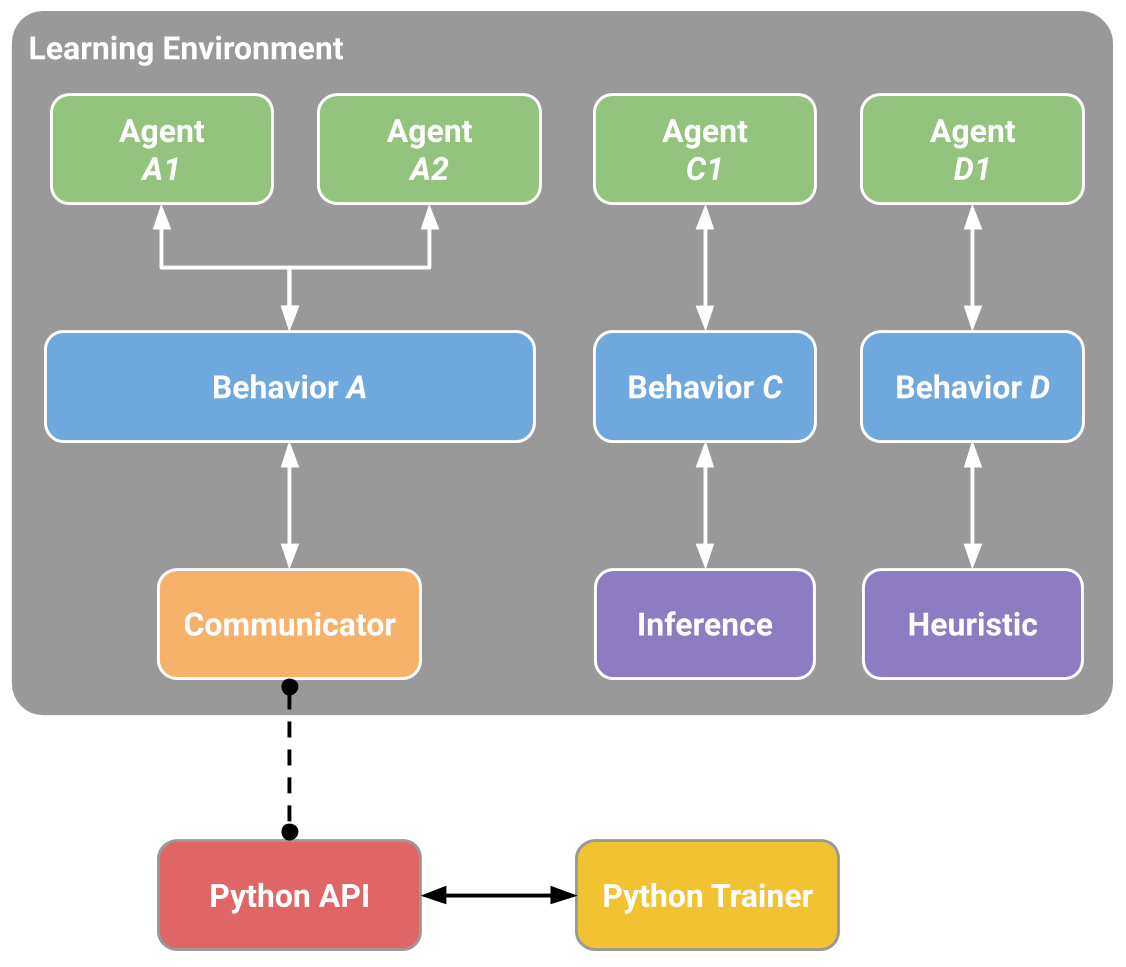
\includegraphics[width=10cm]{figures/learning_environment_example.png}
    \caption[Diagrama de bloques del entorno de ML-Agents]{Diagrama de bloques del entorno de ML-Agents. (Fuente: \cite{ml-agents-github})}
    \label{fig:ml-agents-diagram}
\end{figure}

\newpage

\subsection{ML-Agents en la interfaz de Unity}

En esta sección se resumen los componentes que se deben implementar para crear un entorno de aprendizaje desde la interfaz de Unity. Este TFG no pretende ser una guía de Unity, por lo que no se explica la interfaz en sí. En caso de necesitar más información sobre Unity, se recomienda consultar la documentación oficial \cite{unity-docs}.

Lo primero es crear un entorno con el que interactuará el agente. Este entorno no necesita implementar nada específico de ML-Agents, por lo que el usuario es libre de diseñar cualquier tipo de entorno, utilizando las herramientas habituales de Unity.

El elemento que realmente permite formar un entorno de aprendizaje es la clase \texttt{Agent}. Los \texttt{Game Objects} que se quieran utilizar como agentes deben tener vinculado un \texttt{C\# Script} que extienda esta clase, e implementar los siguientes métodos:
\begin{enumerate}
    \item[-] \texttt{OnEpisodeBegin()}, utilizado para restablecer el agente a unas condiciones iniciales de cada episodio.
    \item[-] \texttt{CollectObservations()}, utilizado para añadir determinadas observaciones del agente a un vector de observaciones.
    \item[-] \texttt{OnActionReceived()}, utilizado para especificar el comportamiento del agente en un paso, basado en las acciones recibidas como parámetro, las cuales proceden ya sea cel modelo que se está entrenando, de la inferencia de un modelo ya entrenado o de una heurística definida por el usuario.
    \item[-] \texttt{Heuristic()}, utilizado para especificar el comportamiento del agente manualmente, modificando las acciones pertinentes.
    \item[-] \texttt{AddReward()}, utilizado para definir la función de recompensa.
\end{enumerate}

Además de la clase \texttt{Agent}, también se requieren los componentes \texttt{Behavior} \texttt{Parameters} y \texttt{Decision Requester}. En caso de querer grabar demostraciones para utilizarlas en GAIL, es necesario utilizar el componente \texttt{Demonstration Recorder}.

Los parámetros relevantes del componente \texttt{Behavior Parameters} (Figura \ref{fig:behavior-param}) son:
\begin{enumerate}
    \item[-] \texttt{Behavior Name}, el nombre de la política.
    \item[-] \texttt{Vector Observation}, donde se define el tamaño del espacio de observaciones.
    \item[-] \texttt{Actions}, donde se define el tamaño del espacio de acciones, tanto continuas como discretas. Cada acción continua consiste en un valor $a \in \mathbb{R}$ dentro del intervalo $[-1, 1]$. Cada acción discreta consiste en un valor discreto cuyo rango se define con \texttt{Branch Size}. Si por ejemplo una acción discreta tiene $\texttt{Branch Size} = 3$, los valores posibles son 0, 1 y 2.
    \item[-] \texttt{Model}, donde se añade el modelo obtenido tras el entrenamiento.
    \item[-] \texttt{Behavior Type}, utilizado para especificar si el agente debe seguir el comportamiento definido por defecto, por heurística, o por inferencia.
    \item[-] \texttt{Team Id}, utilizado para especificar a qué equipo pertenece un agente, en caso de que haya varios equipos.
\end{enumerate}

\begin{figure}[H]
    \centering
    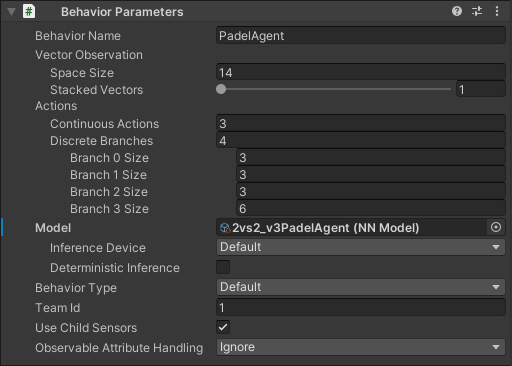
\includegraphics[width=10cm]{figures/behavior-param.png}
    \caption{Ejemplo del componente \texttt{Behavior Parameters} en Unity. (Elaboración propia)}
    \label{fig:behavior-param}
\end{figure}

El \texttt{Decision Requester} (Figura \ref{fig:decision-req}) se utiliza para definir la frecuencia en la que se efectúan las decisiones sobre qué acción realizar tras procesar las observaciones. Por ejemplo, si $\texttt{Decision Period = 5}$, el agente observa y recibe acciones de la política cada 5 \texttt{Fixed Updates} de Unity. Normalmente, el valor del intervalo de tiempo fijo es de 0.02 segundos, por lo que la frecuencia sería de 0.1 segundos.

\begin{figure}[H]
    \centering
    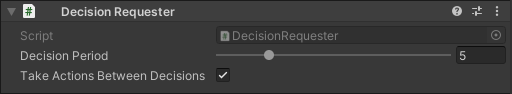
\includegraphics[width=10cm]{figures/decision-req.png}
    \caption{Ejemplo del componente \texttt{Decision Requester} en Unity. (Elaboración propia)}
    \label{fig:decision-req}
\end{figure}

El componente {Demonstration Recorder} (Figura \ref{fig:demo-recorder}) permite la grabación de las demostraciones necesarias para el aprendizaje por imitación. Cuando se graba una demostración, se asume que las acciones son realizadas por expertos, dadas ciertas observaciones. En este componente se define el número de pasos que se quieren grabar, y es posible indicar un número indefinido de pasos mediante el valor 0. También es necesario especificar el nombre del archivo y el directorio en el que se quiera guardar la demostración. Cuando se graban demostraciones en un entorno multi-agente, basta con añadir todas las demostraciones en un mismo directorio, ya que los métodos de aprendizaje por imitación utilizan todas las demostraciones incluidas en el directorio especificado.

\begin{figure}[H]
    \centering
    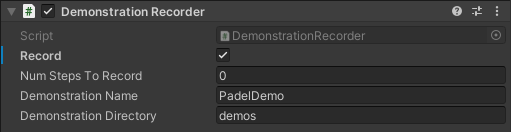
\includegraphics[width=10cm]{figures/demonstration-recorder.png}
    \caption{Ejemplo del componente \texttt{Demonstration Recorder} en Unity. (Elaboración propia)}
    \label{fig:demo-recorder}
\end{figure}

\subsection{Métodos de entrenamiento implementados en ML-Agents}

Los principales algoritmos de aprendizaje por refuerzo disponibles en ML-Agents son Proximal Policy Optimization (PPO) y Soft Actor-Critic (SAC). Entre estos dos, se ha optado por utilizar PPO, ya que se ha demostrado que es un método más genérico y estable que otros algoritmos de RL. Además, citando directamente desde la documentación de ML-Agents: <<\emph{Self-play can be used with our implementations of both Proximal Policy Optimization (PPO) and Soft Actor-Critic (SAC). However, from the perspective of an individual agent, these scenarios appear to have non-stationary dynamics because the opponent is often changing. This can cause significant issues in the experience replay mechanism used by SAC. Thus, we recommend that users use PPO}>>, PPO parece funcionar mejor con \emph{Self-Play}, una funcionalidad que se utiliza para entrenar agentes en juegos adversariales.

Para la parte de aprendizaje por imitación, que en realidad no deja de ser aprendizaje por refuerzo, pero con una extensión en la definición de recompensas, se explora el uso de Generative Adversarial Imitation Learning, el cual utiliza un enfoque adversarial para atribuir recompensas al agente por tener un comportamiento similar a un conjunto de demostraciones. También se ha considerado el uso de Behavioral Clonning, pero al ser un método que se limita a enseñar al agente a copiar exactamente las demostraciones proporcionadas, y al tener un entorno de pádel un espacio de estados muy complejo, no es posible ofrecer un conjunto de demostraciones lo suficientemente grande como para poder generalizar el comportamiento del agente, por lo que se ha descartado.

ML-Agents también dispone de métodos adicionales que pueden ser de utilidad para entrenar agentes en un tipo de entorno específico. Entre estos, los métodos relevantes son Self-Play, utilizado en entornos multi-agente competitivos, y MultiAgent Posthumous Credit Assignment (MA-POCA) \cite{cohen2022use}, utilizado en entornos multi-agente cooperativo, al ser el pádel un deporte que combina cooperación con competición. Sin embargo, se ha descartado el uso de MA-POCA al ser un algoritmo implementado en el contexto de entornos multi-agente, cuya teoría no se cubre en este TFG. Self-Play, por otra parte, es una funcionalidad compatible con PPO por lo que no es necesario orientar la implementación del entorno hacia un entorno multi-agente.

Aunque esto último parece ser contradictorio, ya que tiene sentido que el pádel sea un entorno multi-agente, en realidad, este TFG se centra más bien en entornos de agentes individuales, en los que la cooperación entre agentes acaba surgiendo como una consecuencia del entrenamiento y de la manera en la que se asignan las recompensas, a nivel individual o grupal, según cómo se hayan definido.

\subsubsection{Proximal Policy Optimization}

Proximal Policy Optimization (PPO) \cite{schulman2017proximal}, desarrollado por OpenAI, es un método de gradiente de política que busca mejorar la estabilidad del entrenamiento de agentes, evitando actualizaciones demasiado grandes en la política.

Se sabe, empíricamente, que es más probable converger hacia una solución óptima cuando la política varía poco entre actualizaciones. Cuando el paso del gradiente es demasiado grande, se corre el riesgo de empeorar la política, haciendo que sea díficil o incluso imposible recuperar su bondad.

\newpage

Para actualizar la política de manera conservativa, PPO introduce una función que limita el cambio de la política, llamada función objetivo sustituta con límite (\emph{clipped surrogate objective function}), denominada sustituta en el sentido de que es una aproximación de la función objetivo real (maximizar el retorno esperado), ya que no aplica directamente el gradiente, sin límite (como en los métodos \emph{vanilla}), que teóricamente conllevaría a conseguir una política óptima.

En esta función, se sustituye la probabilidad logarítmica de la función objetivo del teorema del gradiente de política con ventaja (Ecuación \ref{a2c}), por una relación de probabilidad definida como
\begin{equation}
    r_t(\theta) = \frac{\pi_\theta(a_t|s_t)}{\pi_{\theta_{\text{old}}}(a_t|s_t)}
\end{equation}
la cual calcula la relación entre la política actual $\pi_\theta(a_t|s_t)$ y la política anterior $\pi_{\theta_{\text{old}}}(a_t|s_t)$. Sustituyendo esta relación en la función objetivo, y restringiendo el cambio de la política en un pequeño rango, se obtiene la función objetivo sustituta con límite:
\begin{equation}
    L^{CLIP}(\theta) = \hat{\mathbb{E}}\Bigl[\min(r_t(\theta)\hat{A}_t,\text{ clip}(r_t(\theta), 1-\epsilon, 1+\epsilon)\hat{A}_t)\Bigr]
\end{equation}
donde $\epsilon$ es un hiperparámetro, generalmente pequeño (e.g $\epsilon=0\text{.}2)$. El primer término dentro de la función de minimización, $r_t(\theta)\hat{A}_t$, es el objetivo sustituto sin límite. El segundo término, $\text{clip}(r_t(\theta), 1-\epsilon, 1+\epsilon)\hat{A}_t$, modifica el objetivo sustituto limitando la relación $r_t(\theta)$ dentro del intervalo $[1-\epsilon, 1+\epsilon]$. Al escoger finalmente el mínimo entre estos dos términos, el objetivo final acaba siendo una cota inferior del objetivo sustituto sin límite, evitando de esta manera cambios excesivamente grandes en la política.

\begin{figure}[H]
    \centering
    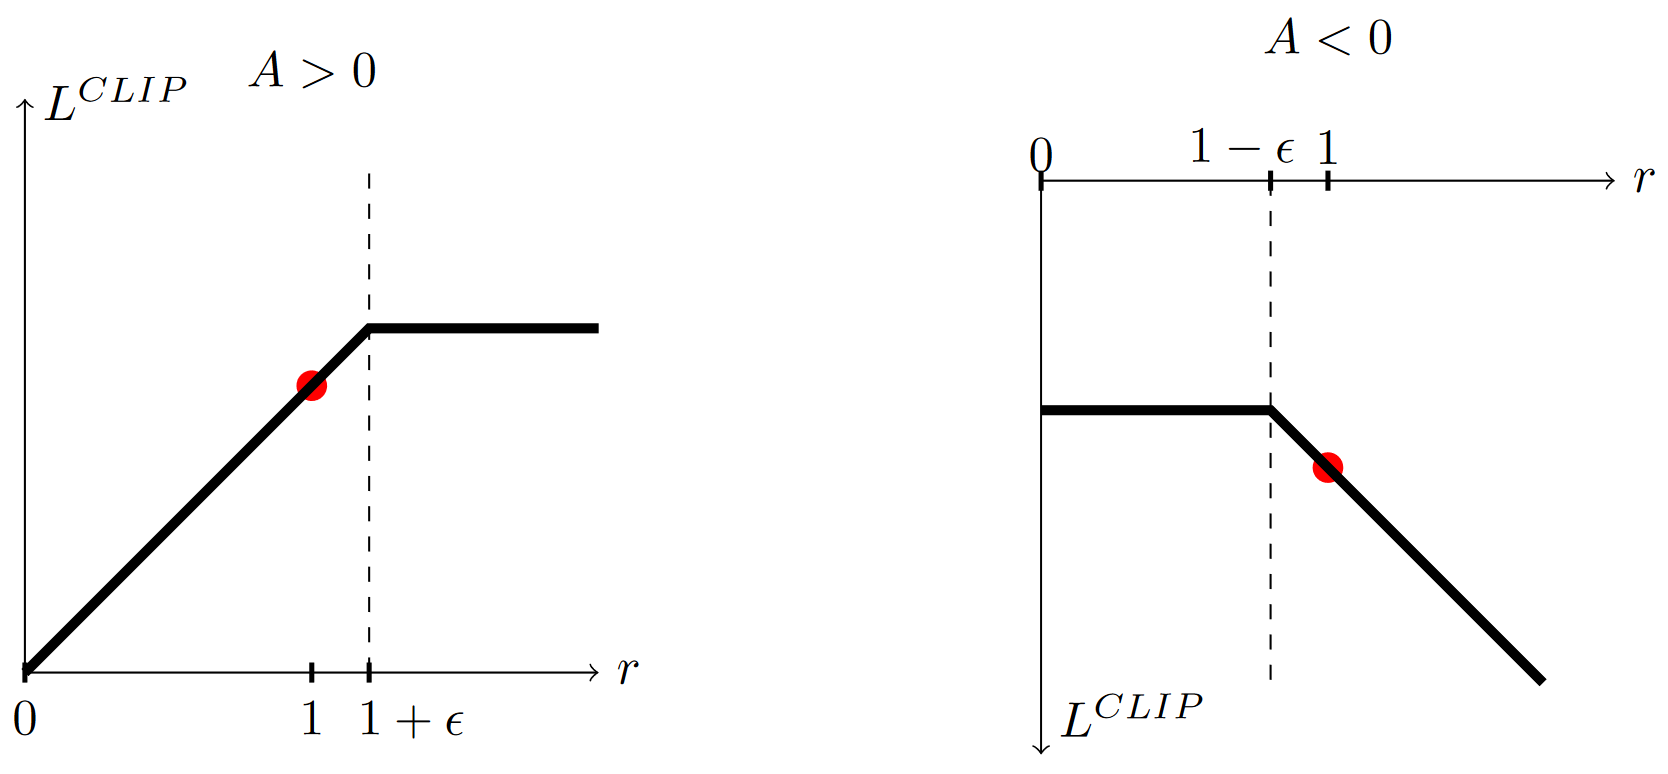
\includegraphics[width=12.5cm]{figures/ppo.png}
    \caption[Gradiente de la función sustituto $L^{CLIP}$]{Paso del gradiente de la función sustituto $L^{CLIP}$ en función de la relación $r_t(\theta)$, para ventajas positivas (izquierda) y negativas (derecha). (Fuente: \cite{schulman2017proximal})}
    \label{fig:ppo}
\end{figure}

\begin{table}[H]
    \centering
    \begin{tabular}{|>{\rowmac}c|>{\rowmac}c|>{\rowmac}c|>{\rowmac}c|>{\rowmac}c|>{\rowmac}c<{\clearrow}|}
        \hline
        \setrow{\bfseries} $r_t(\theta) > 0$ & $\hat{A}_t$ & \makecell{Valor de \\ $min$} & \makecell{Objetivo \\ limitado} & \makecell{Signo del \\ objetivo} & Gradiente \\ \hline\hline
        $r_t(\theta) \in [1 - \epsilon, 1 + \epsilon]$ & $+$ & $r_t(\theta)\hat{A}_t$ & no & $+$ & \checkmark \\
        \hline
        $r_t(\theta) \in [1 - \epsilon, 1 + \epsilon]$ & $-$ & $r_t(\theta)\hat{A}_t$ & no & $-$ & \checkmark \\
        \hline
        $r_t(\theta) < 1 - \epsilon$ & $+$ & $r_t(\theta)\hat{A}_t$ & no & $+$ & \checkmark \\
        \hline
        $r_t(\theta) < 1 - \epsilon$ & $-$ & $(1-\epsilon)\hat{A}_t$ & sí & $-$ & 0 \\
        \hline
        $r_t(\theta) > 1 + \epsilon$ & $+$ & $(1+\epsilon)\hat{A}_t$ & sí & $+$ & 0 \\
        \hline
        $r_t(\theta) > 1 + \epsilon$ & $-$ & $r_t(\theta)\hat{A}_t$ & no & $-$ & \checkmark \\
        \hline
    \end{tabular}
    \caption[Resumen del comportamiento de la función objetivo sustituto con límite $L^{CLIP}$]{Resumen del comportamiento de la función objetivo sustituto con límite $L^{CLIP}$. (Fuente: \cite{danielbickppo})}
    \label{tab:casos-clip}
\end{table}

En la Figura \ref{fig:ppo} se muestra el cambio en el gradiente del valor de $L^{CLIP}$ en función de la relación $r_t(\theta)$, donde se dan seis casos no triviales (esto es, cuando $r_t(\theta) > 0$), distinguidos en la Tabla \ref{tab:casos-clip}:
\begin{enumerate}
    \item Cuando la relación se encuentra dentro del intervalo del límite y la ventaja es positiva, se aplica un gradiente positivo para aumentar la probabilidad de una determinada acción.
    \item Igual que en el primer caso, cuando se encuentra dentro del intervalo del límite y la ventaja es negativa, se aplica un gradiente negativo para decrementar la probabilidad de una determinada acción.
    \item Cuando la relación es inferior al intervalo del límite y la ventaja es positiva (actualmente cierta acción es menos probable que en la política anterior pero genera más recompensas), se aplica un gradiente positivo para aumentar la probabilidad de una determinada acción.
    \item Cuando la relación es inferior al intervalo del límite y la ventaja es negativa (actualmente cierta acción es menos probable que en la política anterior y genera menos recompensas), al ya tener la política actual una menor probabilidad de realizar una determinada acción, no es necesario decrementar aún más su probabilidad, por lo que el gradiente es 0.
    \item Cuando la relación es superior al intervalo del límite y la ventaja es positiva (actualmente cierta acción es más probable que en la política anterior y genera más recompensas), al ya tener la política actual una mayor probabilidad de realizar una determinada acción, no es necesario aumentar aún más su probabilidad, por lo que el gradiente es 0.
    \item Cuando la relación es superior al intervalo del límite y la ventaja es negativa (actualmente cierta acción es más probable que en la política anterior pero genera menos recompensas), se aplica un gradiente negativo para decrementar la probabilidad de una determinada acción.
\end{enumerate}
En resumen, dentro del intervalo del límite (casos 1 y 2), el cambio de la política es pequeño así que es seguro realizar el gradiente según la ventaja. Cuando la relación está fuera del intervalo del límite: si la política actual se contradice con la ventaja (casos 3 y 6), se aplica el gradiente según la ventaja; si la política actual coincide con la ventaja (casos 4 y 5), no se aplica ningún gradiente ya que no es necesario modificarla.

Cabe destacar que PPO se puede utilizar junto a métodos actor-crítico. Cuando las arquitecturas de redes neuronales del actor (política) y el crítico (función de valor) comparten parámetros $\theta$, como es en el caso de la implementación de PPO en ML-Agents, se utiliza una función de pérdida que combina la función objetivo sustituto con límite y un término de error de la función de valor. Para tratar de incentivar la exploración, también es posible añadir un bono de entropía, de manera que cuanta más incerteza haya en la distribución de probabilidades, mayor será el bono. Combinando estos términos, se obtiene la siguiente función objetivo, la cual se debe maximizar:
\begin{equation}
    L_t^{CLIP+VF+S}(\theta) = \hat{\mathbb{E}}_t \left[ L_t^{CLIP}(\theta) - c_1 L_t^{V F}(\theta) + c_2 H[\pi_\theta](s_t) \right]
\end{equation}
donde $c_1$ y $c_2$ son coeficientes, $L_t^{VF}(\theta)$ es una función de pérdida del error cuadrático $(V_\theta(s_t)-V_t^{targ})^2$, y $H$ el bono de entropía.

\newpage

\subsubsection{Recompensas extrínsecas e intrínsecas}

Las recompensas que puede recibir un agente están definidas, típicamente, en el propio entorno, y se asocian con alcanzar un cierto objetivo. En general, estas recompensas se conocen como recompensas extrínsecas desde el punto de vista de los algoritmos de aprendizaje.

Además de las recompensas extrínsecas, las recompensas también se pueden definir fuera del entorno, denominadas recompensas intrínsecas, y son aquellas que provienen el propio algoritmo de aprendizaje, para incentivar al agente a comportarse de una cierta manera. GAIL, por ejemplo, define una recompensa intrínseca que el agente obtiene dependiendo de la similitud entre el comportamiento del agente y las demostraciones proporcionadas. Durante el entrenamiento, el agente busca maximizar la combinación de recompensas extrínsecas e intrínsecas.

\subsubsection{Curiosity}

En la primera parte de este capítulo, en el estudio del aprendizaje por refuerzo, se asumía que cada interacción del agente con el entorno conllevaba a conseguir una recompensa. Sin embargo, hay entornos en los que el agente raramente recibe recompensas, por lo que le es imposible saber si una acción ha sido buena o no. A este problema se le conoce como \emph{reward-sparsity} (escasez de recompensas).

Cuando un agente no obtiene \emph{feedback} sobre cómo está actuando, es muy probable que acabe moviéndose sobre un mismo conjunto de estados durante mucho tiempo hasta hallar, si hay suerte, un estado que le proporcione recompensas. En escenarios donde hay escasez de recompensas, el uso de recompensas intrínsecas puede ser de gran ayuda.

Curiosity \cite{pathak2017curiosity} es un algoritmo que ayuda al agente a descubrir nuevos estados de un entorno por pura curiosidad, otorgándole una recompensa intrínseca cuando las recompensas extrínsecas son escasas o incluso inexistentes. Internamente, consiste en un Módulo de Curiosidad Intrínseca (ICM), mostrado en la Figura \ref{fig:icm}, el cual entrena dos modelos de redes neuronales profundas:

\begin{enumerate}
    \item[-] El \emph{Inverse Model}, cuyo fin es predecir la acción $a_t$ que ha realizado el agente para moverse de un estado $s_{t}$ al estado siguiente $s_{t+1}$, utilizando una red neuronal para aprender la función $g$, definida como \begin{equation}
        \hat{a}_t = g\Bigl(s_t, s_{t+1};\theta_I\Bigr)
    \end{equation} donde $\hat{a}_t$ es la estimación prevista y $\theta_I$ son los parámetros de la red neuronal que se entrenan para optimizar una función de pérdida $L_I$, la cual mide la discrepancia entre la acción estimada y la acción real:
    \begin{equation}
        \min_{\theta_I} L_I(\hat{a}_t, a_t)
        \label{inverse-loss}
    \end{equation}
    Además, este modelo tiene un paso intermedio en el que se codifican los estados $s_t$ y $s_{t+1}$ en vectores de características $\phi(s_t)$ y $\phi(s_{t+1})$. De esta manera, al minimizar la discrepancia entre las acciones $a_t$ y $\hat{a}_t$, se obtiene un submódulo capaz de extraer las características más relevantes de cada estado, es decir, aquellas características que realmente han llevado al agente a moverse de un estado $s_t$ al estado siguiente $s_{t+1}$ realizando la acción $a_t$.
    \newpage
    \item[-] El \emph{Forward Model}, cuyo fin es predecir la codificación del estado siguiente $\phi(s_{t+1})$ dada una acción $a_t$ y la codificación de un estado actual $\phi(s_t)$, también utilizando una red neuronal para aprender la función $f$, definida como
    \begin{equation}
        \hat{\phi}(s_{t+1}) = f\Bigl(\phi(s_t), a_t;\theta_F\Bigr)
    \end{equation} donde $\hat{\phi}(s_{t+1})$ es la estimación prevista de $\phi(s_{t+1})$ y $\theta_F$ los parámetros de la red neuronal que se optimizan minimizando la función de pérdida $L_F$, definida como la norma $L^2$ (norma euclídea) al cuadrado entre la codificación estimada y la codificación real:
    \begin{equation}
        L_F\Bigl(\phi(s_{t+1}), \hat{\phi}(s_{t+1})\Bigr) = \frac{1}{2}\Vert\hat{\phi}(s_{t+1}) - \phi(s_{t+1})\Vert_{2}^{2}
        \label{eq:forward-loss}
    \end{equation}
\end{enumerate}

Optimizando ambos modelos conjuntamente, el \emph{Inverse Model} aprende un espacio de características que codifica únicamente la información relevante para predecir las acciones del agente, y el \emph{Forward Model} hace predicciones en este espacio de características.

Utilizando las funciones entrenadas $g$ y $f$ se genera una recompensa intrínseca basada en la curiosidad $r_t^i$, la cual se define también como la norma $L^2$ al cuadrado entre la codificación estimada y la codificación real:

\begin{equation}
    r_t^i = \frac{\eta}{2}\Vert \hat{\phi}(s_{t+1})-\phi(s_{t+1})\Vert_2^2
\end{equation}
donde $\eta > 0$ es un factor de escala. De esta manera, cuanto menos se parezca la codificación del estado siguiente esperado $\hat{\phi}(s_{t+1})$ a la codificación del estado siguiente real $\phi(s_{t+1})$, mayor será la recompensa intrínseca. Gracias a que el espacio de características no tiene incentivos para codificar elementos del estado que no tienen influencia en las acciones del agente, el agente no recibe ninguna recompensa cuando se encuentra en estados que en su totalidad parecen distintos, pero esencialmente son iguales. Esto hace que la estrategia de exploración sea robusta frente a la presencia de ruido en el entorno, ya sea por cambios de iluminación, objetos distractores, etc.

El problema conjunto de optimización se compone por las funciones de pérdida de las Ecuaciones \ref{eq:forward-loss} y \ref{inverse-loss}, las cuales se deben minimizar conjuntamente, junto al objetivo principal de maximización del retorno:
\begin{equation}
    \min_{\theta_P, \theta_I, \theta_F} \left[- \lambda\mathbb{E}_{\pi(s_t;\theta_P)}\Bigl[\sum_t r_t\Bigr]+(1-\beta)L_I+\beta L_F \right]
\end{equation}
donde $0 \leq \beta \leq 1$ es un escalar que pondera la pérdida del modelo inverso frente a la pérdida del modelo directo, y $\lambda > 0$ es un escalar que pondera la importancia del gradiente de la política frente a la importancia de la recompensa intrínseca.

\begin{figure}[H]
    \centering
    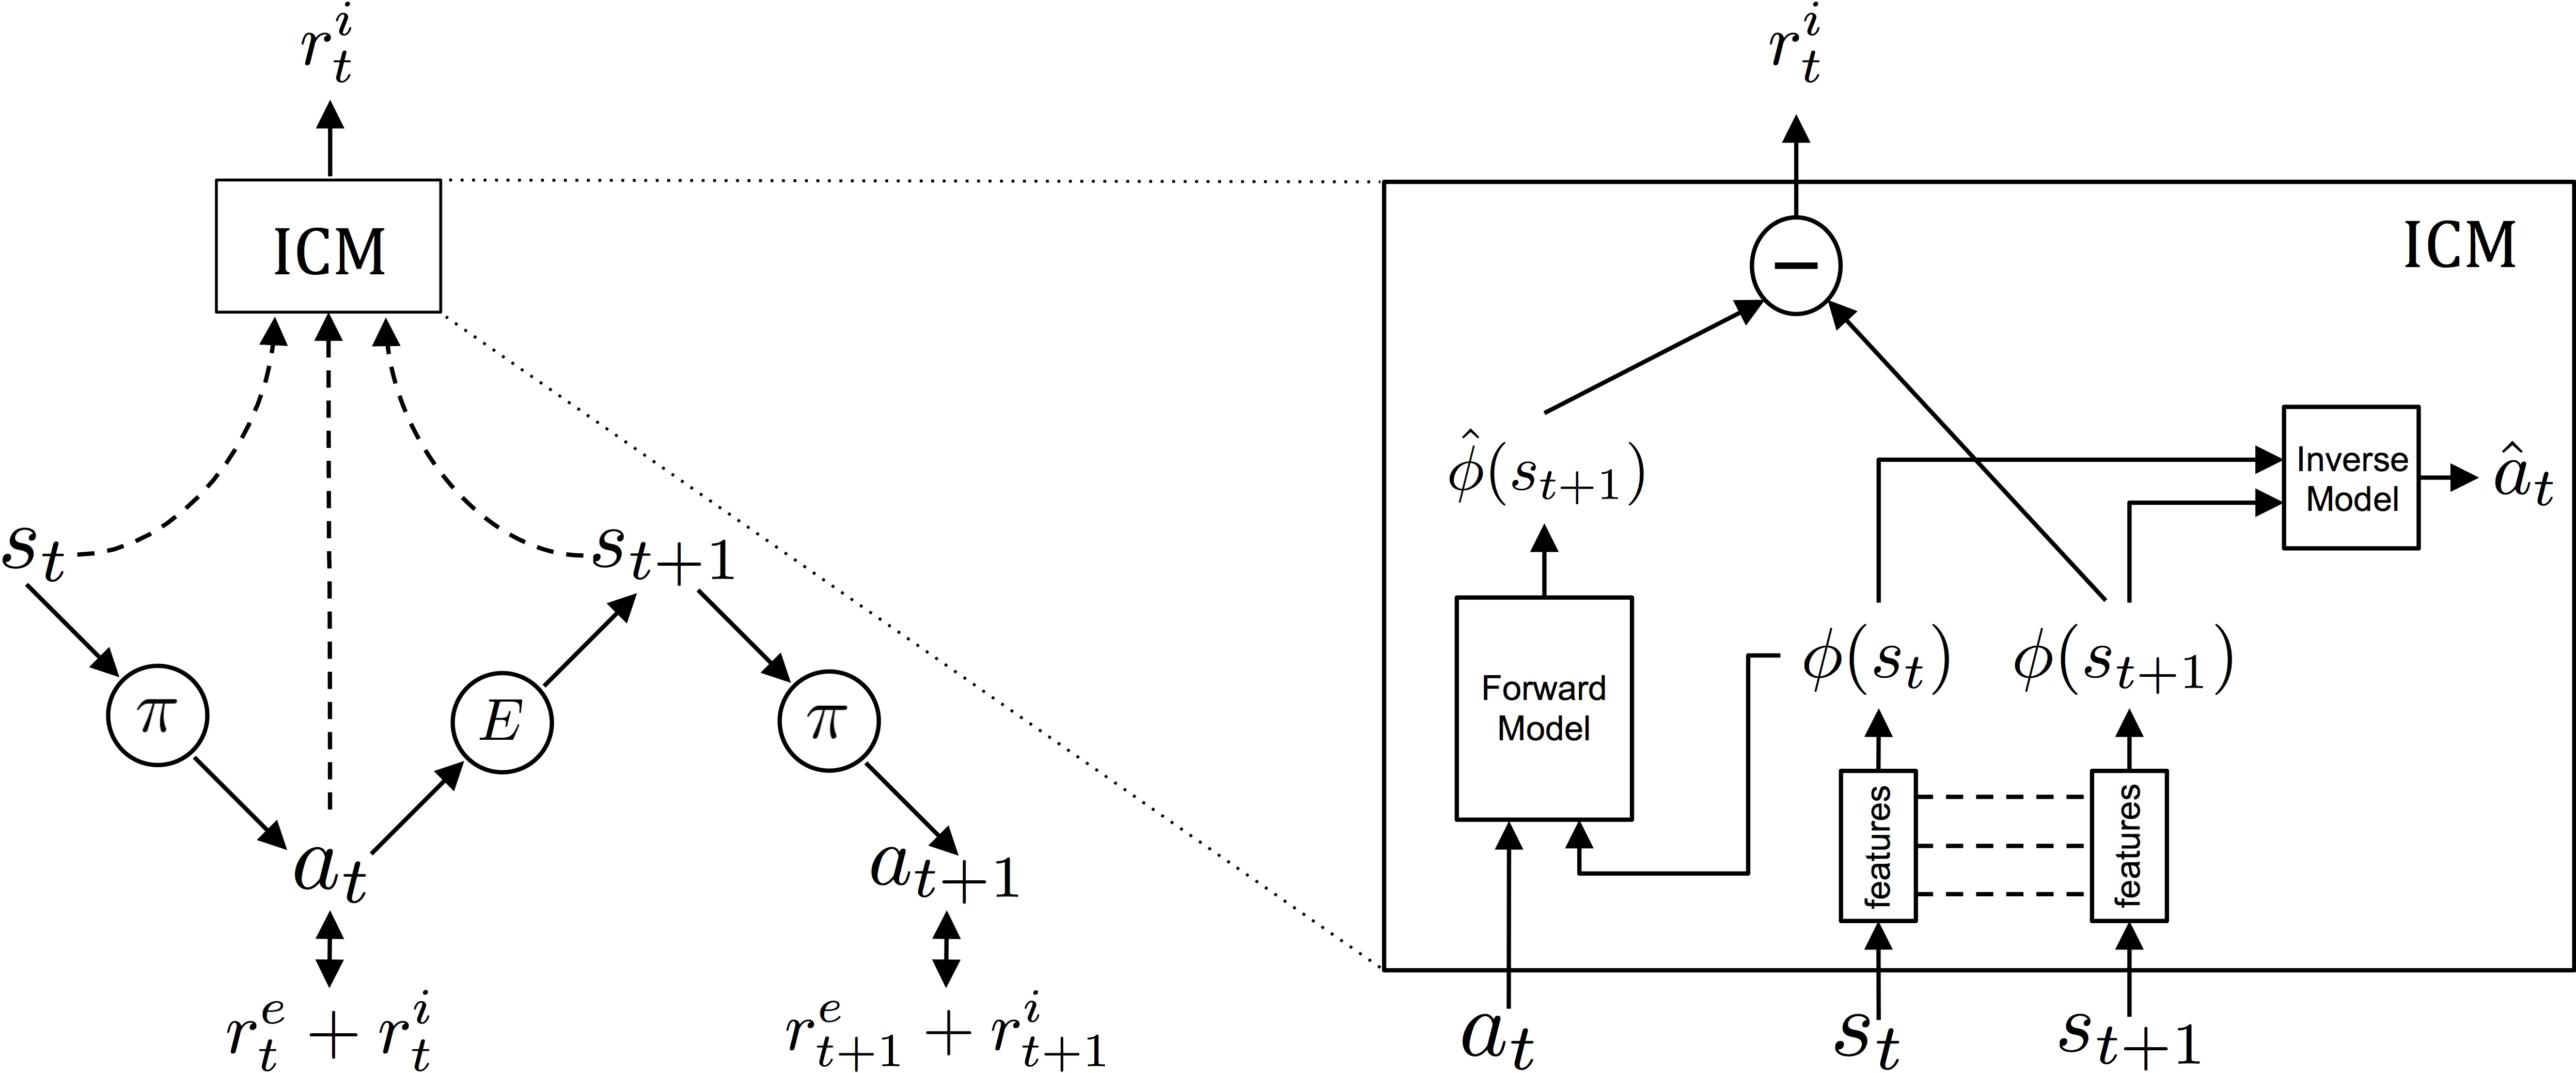
\includegraphics[width=15cm]{figures/curiosity.jpg}
    \caption[Módulo de Curiosidad Intrínseca (ICM)]{Módulo de Curiosidad Intrínseca (ICM). (Fuente: \cite{pathak2017curiosity})}
    \label{fig:icm}
\end{figure}

\subsubsection{Generative Adversarial Imitation Learning}

Generative Adversarial Imitation Learning (GAIL) \cite{ho2016generative} es un algoritmo que combina las ideas del aprendizaje por refuerzo inverso (IRL), uno de los enfoques del aprendizaje por imitación, y las redes generativas antagónicas (GAN). Debido a que tanto IRL como GAN son temas que están fuera del marco teórico de este TFG, en este apartado no se hace un estudio exhaustivo pero sí se da una intuición sobre GAIL.

En el aprendizaje por refuerzo tradicional, el objetivo es aprender una política para maximizar una función de recompensa predefinida en el entorno. En el aprendizaje por refuerzo inverso, se le da una vuelta a este problema y el objetivo pasa a ser definir una función de recompensa a partir de la observación del comportamiento de un agente.

El IRL puede ser útil en entornos en los que es difícil predefinir una función de recompensa, debido a la complejidad del entorno. Para ello, se introduce la idea de utilizar muestras de agentes expertos, denominadas demostraciones, las cuales se asumen que siguen un comportamiento óptimo en un determinado entorno. Utilizando estas muestras, el agente adopta el rol de aprendiz y trata de aprender una política lo más parecida posible a la del experto. Para guiar al agente aprendiz durante el proceso de entrenamiento, el modelo de IRL determina en qué situaciones debe recompensar al agente aprendiz, según el grado de similitud con el comportamiento del agente experto.

Uno de los enfoques de IRL consiste en utilizar GAN. En una arquitectura de GAN se entrenan dos modelos simultáneamente: un modelo generativo $G$, que aprende una distribución de datos, y un modelo discriminador $D$, que predice si una muestra de entrada procede de conjunto de muestras reales, o bien del generador $G$. Mientras que el discriminador se entrena para hacer una distinción correcta entre si una muestra de entrada proviene del generador o del conjunto de muestras reales, el generador intenta engañar al discriminador haciéndole pensar que las muestras que genera son reales. Entrenando ambos modelos simultáneamente, el objetivo final es conseguir que el generador sea capaz de crear muestras cuya distribución de datos sea la misma que la de las muestras reales.

\newpage

El uso de GAN en el contexto de IRL da lugar a GAIL. En GAIL, el discriminador debe aprender a distinguir si una observación/acción procede de una demostración o del generador, es decir, del agente aprendiz. De esta manera, durante el entrenamiento, mientras el agente va mejorando cada vez más, recibiendo recompensas intrínsecas según cuánto se acerque su comportamiento a las demostraciones expertas, el discriminador se va volviendo cada vez más estricto haciendo que el agente se deba esforzar más para engañarle.

Una de las ventajas de GAIL es que, en lugar de buscar replicar exactamente el comportamiento del agente experto, permite aprender una política que produzca acciones y estados similares a las demostraciones, es decir, una aproximación, requiriendo menos demostraciones para conseguir una política más genérica.

\subsubsection{Self-play}

En entornos en los que varios agentes compiten entre sí, entrenar una política correctamente no resulta fácil. Por una parte, es necesario tener un oponente bien entrenado para jugar contra el agente a ser entrenado. Por otra, cuando un oponente es demasiado bueno, es difícil que el agente mejore su política cuando está perdiendo constantemente y no tiene control sobre lo que está ocurriendo.

Una forma de hacer frente a este problema es utilizar oponentes con el mismo nivel que el agente, y que vayan mejorando simultáneamente a medida que compiten. En el contexto de RL, a este mecanismo se le llama \emph{self-play} \cite{self-play}.

En self-play, la idea es que los agentes compartan copias de la misma política, ya que todos tratan de resolver el mismo problema. En un entorno de uno contra uno, uno de los agentes fija su política (agente a entrenar) mientras que el otro la va cambiando (agente oponente). A medida que entrenan, el oponente va cambiando de política a copias más recientes de la política que está aprendiendo el agente a entrenar. De esta manera, la política va mejorando progresivamente a la vez que el oponente va incrementando su complejidad. Por supuesto, este mecanismo se puede extender a entornos de más agentes, por ejemplo de dos contra dos, mediante el uso de equipos.

\subsection{Configuración del entrenamiento}

Por último, en sección se recopila la configuración relevante del entrenamiento de agentes en ML-Agents, explicando  el funcionamiento de los parámetros e hiperparámetros que se utilizan en los métodos de entrenamiento presentados en la sección anterior. Una explicación más detallada de todos los parámetros, inluidos aquellos que se omiten en esta sección, puede consultarse en la documentación de ML-Agents \cite{ml-agents-config-file}.

\subsubsection{Configuración común}

\begin{table}[H]
\centering
    \begin{tabular}{|>{\rowmac}p{3.5cm}|>{\rowmac}p{10cm}<{\clearrow}|} 
        \hline
        \multicolumn{1}{|c|}{\textbf{Ajuste}} & \multicolumn{1}{c|}{\textbf{Descripción}} \\ \hline \hline
        \texttt{trainer\_type} & Tipo de entrenamiento a utilizar: \texttt{ppo}, \texttt{sac} o \texttt{poca}. \\
        \hline
        \texttt{summary\_freq} & Número de experiencias que deben ser procesadas antes de generar y mostrar estadísticas del entrenamiento. \\
        \hline
        \texttt{max\_steps} & Número total de pasos que deben realizarse en el entorno antes de terminar el entrenamiento. \\
        \hline
        \texttt{keep\_checkpoints} & Número de puntos de guardado del modelo que se deben guardar. \\
        \hline
        \texttt{even\_checkpoints} & Indica si los puntos de guardado deben distribuirse uniformemente, dependiendo de los valores de \texttt{keep\_checkpoints} y \texttt{max\_steps} \\
        \hline
        \texttt{hyperparameters/ learning\_rate} & Factor de aprendizaje inicial utilizado en el descenso de gradiente. \\
        \hline
        \texttt{hyperparameters/ learning\_rate\_ schedule} & Determina cómo cambia el factor de aprendizaje con el tiempo. Para PPO se recomienda una decadencia lineal, para una convergencia más estable. Los valores posibles son \texttt{linear} o \texttt{constant}\\
        \hline
        \texttt{hyperparameters/ batch\_size} & Número de experiencias utilizadas en cada iteración del descenso de gradiente. \\
        \hline
        \texttt{hyperparameters/ buffer\_size} & En PPO, corresponde al número de experiencias que deben ser guardadas antes de actualizar la política. \\
        \hline
        \texttt{network\_settings/ num\_layers} & Número de \emph{hidden layers} de la red neuronal, tanto para la red neuronal del actor como la del crítico. \\
        \hline
        \texttt{network\_settings/ hidden\_units} & Número de neuronas de cada \emph{hidden layer}, tanto para la red neuronal del actor como la del crítico. \\
        \hline
    \end{tabular}
    \caption[Configuración común de todos los tipos de entrenamiento (PPO, SAC y POCA)]{Configuración común de todos los tipos de entrenamiento (PPO, SAC y POCA). (Fuente: \cite{ml-agents-config-file})}
    \label{tab:config-general}
\end{table}

\subsubsection{Configuración específica de PPO}

\begin{table}[H]
\centering
    \begin{tabular}{|>{\rowmac}p{3.5cm}|>{\rowmac}p{10cm}<{\clearrow}|} 
        \hline
        \multicolumn{1}{|c|}{\textbf{Ajuste}} & \multicolumn{1}{c|}{\textbf{Descripción}} \\ \hline \hline
        \texttt{hyperparameters/ beta} & Factor de escala del bono de entropía.\\
        \hline
        \texttt{hyperparameters/ epsilon} & Determina el límite de divergencia entre la política actual y la anterior durante el cálculo de descenso de gradiente. \\
        \hline
        \texttt{hyperparameters/ beta\_schedule} & Determina cómo cambia \texttt{beta} con el tiempo. \\
        \hline
        \texttt{hyperparameters/ epsilon\_schedule} & Determina cómo cambia \texttt{epsilon} con el tiempo.\\
        \hline
        \texttt{hyperparameters/ num\_epoch} & Número de veces que se recorre el búfer de experiencias al realizar la optimización mediente gradiente descendiente. \\
        \hline
    \end{tabular}
    \caption[Configuración específica de PPO]{Configuración específica de PPO. (Fuente: \cite{ml-agents-config-file})}
    \label{tab:config-ppo}
\end{table}

\subsubsection{Recompensas extrínsecas}

\begin{table}[H]
\centering
    \begin{tabular}{|>{\rowmac}p{3.5cm}|>{\rowmac}p{10cm}<{\clearrow}|} 
        \hline
        \multicolumn{1}{|c|}{\textbf{Ajuste}} & \multicolumn{1}{c|}{\textbf{Descripción}} \\ \hline \hline
        \texttt{extrinsic/strength} & Factor de escala de las recompensas extrínsecas. \\
        \hline
        \texttt{extrinsic/gamma} & Factor de descuento de las recompensas futuras procedentes del entrono. \\
        \hline
    \end{tabular}
    \caption[Configuración de las recompensas extrínsecas]{Configuración de las recompensas extrínsecas. (Fuente: \cite{ml-agents-config-file})}
    \label{tab:config-extrinsic}
\end{table}

\subsubsection{Recompensas intrínsicas de Curiosity}

\begin{table}[H]
\centering
    \begin{tabular}{|>{\rowmac}p{3.5cm}|>{\rowmac}p{10cm}<{\clearrow}|} 
        \hline
        \multicolumn{1}{|c|}{\textbf{Ajuste}} & \multicolumn{1}{c|}{\textbf{Descripción}} \\ \hline \hline
        \texttt{curiosity/strength} & Factor de escala de las recompensas generadas por el módulo de curiosidad intrínseca. \\
        \hline
        \texttt{curiosity/gamma} & Factor de descuento de las recompensas futuras. \\
        \hline
        \texttt{curiosity/ network\_settings} & Especificaciones de la red neuronal utilizada por el modelo de curiosidad intrínseca. \\
        \hline
        \texttt{curiosity/ learning\_rate} & Factor de aprendizaje utilizado para actualizar el módulo de curiosidad intrínseca. \\
        \hline
    \end{tabular}
    \caption[Configuración de las recompensas intrínsecas procedentes de Curiosity]{Configuración de las recompensas intrínsecas procedentes de Curiosity. (Fuente: \cite{ml-agents-config-file})}
    \label{tab:config-curiosity}
\end{table}

\subsubsection{Recompensas intrínsecas de GAIL}

\begin{table}[H]
\centering
    \begin{tabular}{|>{\rowmac}p{3.5cm}|>{\rowmac}p{10cm}<{\clearrow}|} 
        \hline
        \multicolumn{1}{|c|}{\textbf{Ajuste}} & \multicolumn{1}{c|}{\textbf{Descripción}} \\ \hline \hline
        \texttt{gail/strength} & Factor de escala de las recompensas de GAIL. \\
        \hline
        \texttt{gail/gamma} & Factor de descuento de las recompensas futuras. \\
        \hline
        \texttt{gail/demo\_path} & Ruta del directorio de los archivos \texttt{.demo}. \\
        \hline
        \texttt{gail/ network\_settings} & Especificaciones de la red neuronal del discriminador de GAIL. \\
        \hline
        \texttt{gail/learning\_rate} & Factor de aprendizaje utilizado para actualizar el discriminador. \\
        \hline
        \texttt{gail/use\_actions} & Determina si el discriminador debe predecir basándose en acciones y observaciones o únicamente observaciones. \\
        \hline
        \texttt{gail/use\_vail} & Habilita el \emph{variational bottleneck} del discriminador de GAIL. Esta opción fuerza al discriminador a aprender una representación más genérica y reducir la tendencia a ser ``demasiado bueno'' prediciendo.  \\
        \hline
    \end{tabular}
    \caption[Configuración de las recompensas intrínsecas procedentes de GAIL]{Configuración de las recompensas intrínsecas procedentes de GAIL. (Fuente: \cite{ml-agents-config-file})}
    \label{tab:config-gail}
\end{table}

\subsubsection{Configuración de Self-Play}

\begin{table}[H]
\centering
    \begin{tabular}{|>{\rowmac}p{3.5cm}|>{\rowmac}p{10cm}<{\clearrow}|} 
        \hline
        \multicolumn{1}{|c|}{\textbf{Ajuste}} & \multicolumn{1}{c|}{\textbf{Descripción}} \\ \hline \hline
        \texttt{save\_steps} & Número de pasos entre los que se hacen copias de la política que se está entrenando. Un valor grande de \texttt{save\_steps} permite cubrir un rango de niveles de habilidad más amplio. \\
        \hline
        \texttt{team\_change} & Número de pasos entre cambios del equipo que aprende. Cuanto más grande es el valor de \texttt{team\_change}, más capaces se vuelven los agentes del equipo que aprende de vencer a los oponentes. Sin embargo, entrenar contra los mismos oponentes durante demasiado tiempo puede causar \emph{overfitting} contra las estrategias de esos oponentes en particular.\\
        \hline
        \texttt{swap\_steps} & Número de \emph{pasos fantasma} entre cambios de la política del oponente. Un \emph{paso fantasma} es un paso dado por un agente con la política fija (que no está aprendiendo), relevante para entornos asimétricos. \\
        \hline
        \texttt{play\_against\_ latest\_model\_ratio} & Probabilidad con la que el agente se enfrentará contra la copia más reciente de la política. Con una probabilidad de $1 - \texttt{play\_against\_latest\_model\_ratio}$, el agente se enfrentará contra una de las copias pasadas, seleccionada aleatoriamente. \\
        \hline
        \texttt{window} & Tamaño de la ventana deslizante de copias pasadas de la política, desde donde se obtiene la política del oponente. Cada vez que se hace una copia nueva, se descarta la más antigua. Un valor grande implica guardar una mayor diversidad de comportamientos del agente. Aprender una política capaz de enfrentarse a una diversidad de oponentes es más difícil, pero a su vez permite obtener una política más robusta. \\
        \hline
    \end{tabular}
    \caption[Configuración de self-play]{Configuración de self-play. (Fuente: \cite{ml-agents-config-file})}
    \label{tab:config-self-play}
\end{table}
